% use no footline.
% \begin{frame}[plain, noframenumbering]{Outline}
% 	\tableofcontents
% \end{frame}
%%%%%%%%%%%%%%%%%%%%%%%%%%%%%%%%%%%%%%%%%%%%%%%%%%%%%%
\section{Hive}



\begin{frame}
\frametitle{Chapter Objectives}

\begin{itemize}
	\item<1-> Query data lakes/HDFS using Hive. \pause
	\item<2-> Introduction to Hive \pause
	\item<3-> Comparing Hive to Traditional databases.
	\item<4-> Hive Components and Architecture. \pause
	\item<5-> Relational Data Analysis with Hive. \pause
	\item<6-> Hive Data Management. \pause
	\item<7-> Hive Optimization. \pause
	\item<8-> Hive Demo. \pause
\end{itemize}

\end{frame}

%%%%%%%%%%%%%%%%%%%%%%%%%%%%%%%%%%%%%%%%%%%%%%%%%%%%%%
\subsection{Query data lakes/HDFS using Hive}
\begin{frame}
	\frametitle{\subsecname}
	\begin{itemize} 
		\item Data lakes and HDFS store vast amounts of petabyte-scale data. \pause
		\item Data analysts require efficient ways to query this data without delving into intricate Map-Reduce programming.\pause
		\item SQL is a commonly used language for data manipulation, embraced by data analysts, developers, and business users worldwide.\pause
		\item Hive, one of the early tools in this field, simplifies data analysis on big data by offering SQL-like querying capabilities for data lakes and HDFS.\pause
		\item There are other tools like Trino/Presto, Snowflake, and Databricks that can be faster for data lake queries, which we will discuss later.\pause
	\end{itemize}
	\end{frame}
%%%%%%%%%%%%%%%%%%%%%%%%%%%%%%%%%%%%%%%%%%%%%%%%%%%%%%

\subsection{Introduction to hive}
\begin{frame}
\frametitle{\subsecname}
\begin{itemize} 
	\item Apache Hive is a powerful data warehousing and SQL-like query language tool within the Hadoop ecosystem.\pause
	\item It was developed by Facebook and later contributed to the Apache Software Foundation, making it an open-source project.\pause
	\item Apache Hive had its initial release on October 1, 2010.	\pause
\end{itemize}
\end{frame}

\begin{frame}
	\frametitle{\subsecname}
	\begin{itemize} 
		\item Hive provides a user-friendly interface to work with and analyze large datasets stored in Hadoop Distributed File System (HDFS) or other compatible storage systems.\pause
		\item With its SQL-like language called HiveQL, users can write queries to extract, transform, and analyze data, making it accessible to a wide range of data professionals\pause
		\item Apache Hive bridges the gap between the world of big data and traditional relational databases, making it a valuable tool for data engineers, analysts, and data scientists.\pause	
	\end{itemize}
	\end{frame}

	\begin{frame}[fragile]
		\frametitle{Hive Query Example}

\begin{lstlisting}[caption={Hive Query Example},language=SQL]
SELECT * 
FROM Customers
WHERE Country = 'USA';
\end{lstlisting}

	\end{frame}
%%%%%%%%%%%%%%%%%%%%%%%%%%%%%%%%%%%%%%%%%%%%%%%%%%%%%%


\subsubsection{Overview of Apache Hive}
\begin{frame}
\frametitle{Overview of Apache Hive}
\begin{itemize} 
	\item Apache Hive is a high-level data warehousing and SQL-like query language tool built on top of MapReduce.\pause
	\item It acts as an abstraction layer, allowing users to work with large datasets stored in Hadoop Distributed File System (HDFS) without needing to write complex MapReduce jobs themselves.\pause
	\item Under the hood, Hive generates MapReduce jobs that are executed on the Hadoop cluster. This means it leverages the distributed processing capabilities of Hadoop for scalability and parallel processing.\pause
	\item Hive has evolved beyond MapReduce to support other execution engines, such as Tez and Spark, which can enhance performance and usability. This will be discussed later.\pause

\end{itemize}
\end{frame}

%%%%%%%%%%%%%%%%%%%%%%%%%%%%%%%%%%%%%%%%%%%%%%%%%%%%%%

\subsubsection{Comparing Hive to Traditional Databases}
\begin{frame}{Comparison between Apache Hive and Traditional RDBMS (Part 1)}
	\begin{table}[h!]
		\centering
		\resizebox{\textwidth}{!}{%
		\begin{tabular}{|m{5cm}|m{6cm}|m{6cm}|}	    
		\hline
		\rowcolor{Gray}
		\textbf{Feature} & \textbf{Apache Hive} & \textbf{Traditional RDBMS} \\
		\hline
		Purpose & Big data analytics. & Transactional systems and traditional data warehousing. \\
		\hline
		Query Language & HiveQL, similar to SQL. & SQL. \\
		\hline
		Speed & Slower, optimized for batch processing. & Faster, optimized for real-time transactional processing. \\
		\hline
		Data Size & Designed to handle petabytes of data. & gigabytes to terabytes; some systems can handle petabytes at higher cost. \\
		\hline
		ACID Properties & Limited ACID support. & Full ACID support. \\
		\hline
	\end{tabular}
	}
	\caption{Comparison between Apache Hive and Traditional RDBMS}
  \end{table}
  \end{frame}
  
  \begin{frame}{Comparison between Apache Hive and Traditional RDBMS (Part 2)}
	\begin{table}[h!]
		\centering
		\resizebox{\textwidth}{!}{%
		\begin{tabular}{|m{5cm}|m{6cm}|m{6cm}|}	  
		\hline
		\rowcolor{Gray}
		\textbf{Feature} & \textbf{Apache Hive} & \textbf{Traditional RDBMS} \\
		\hline
		Storage & Built on HDFS. & Uses internal storage mechanisms. \\
		\hline
		Metadata Storage & Stored in Hive Metastore. & Stored in system catalogs within the database. \\
		\hline
		Compute Engine & MapReduce, Tez, or Spark can be used. & Built-in engine, tightly integrated. \\
		\hline
		Query Execution Location & Executes on Hadoop cluster nodes. & Executes on the database server. \\
		\hline
		Data Storage Formats & ORC, Parquet, CSV, JSON, XML, Avro & Proprietary Binary Format \\
		\hline
		Max Simultaneous Connections & Governed by Hadoop Cluster & Varies (Hundreds to Thousands) \\
		\hline		
	\end{tabular}
	}
	\caption{Comparison between Apache Hive and Traditional RDBMS}
  \end{table}
  \end{frame}
  
%%%%%%%%%%%%%%%%%%%%%%%%%%%%%%%%%%%%%%%%%%%%%%%%%%%%%%

\subsection{Hive Architecture}

\begin{frame}{Abstract Components of Apache Hive}
	\begin{itemize}
		\item Hive Clients.
		\item Hive Services.
		\item Hive Metadata (Metastore).
		\item Storage.
		\item Compute.
	\end{itemize}
	\end{frame}
	
\begin{frame}{Abstract Components of Apache Hive}
	\begin{figure}
		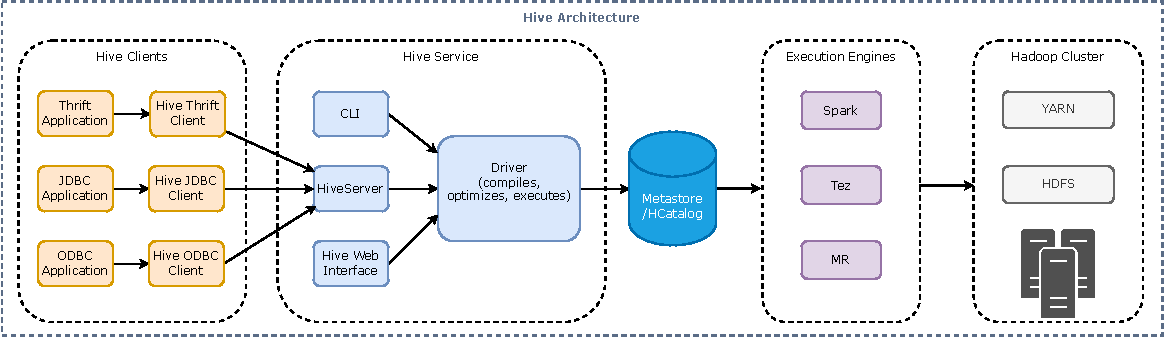
\includegraphics[width=\textwidth,height=\textheight,keepaspectratio]{./Figures/chapter-03/Hive_Architecture.pdf}	
		\caption{Abstract Components of Apache Hive}
	\end{figure}
\end{frame}
%%%%%%%%%%%%%%%%%%%%%%%%%%%%%%%%%%%%%%%%%%%%%%%%%%%%%%
\begin{frame}
\frametitle{Hive Clients}
	\framesubtitle{Connecting with Hive}
	
	\begin{itemize}
	  \item Hive provides various drivers for seamless communication with different types of applications.
	  \item For Thrift-based applications, Hive offers the Thrift client for effective communication.
	  \item If you are working with Java-related applications, Hive provides JDBC drivers for smooth integration.
	  \item Additionally, for other types of applications, Hive offers ODBC drivers, ensuring versatility.
	  \item These clients and drivers serve as intermediaries, connecting your applications with Hive Server in the Hive services.
	\end{itemize}
	
	\end{frame}
%%%%%%%%%%%%%%%%%%%%%%%%%%%%%%%%%%%%%%%%%%%%%%%%%%%%%%
\begin{frame}
	\frametitle{Hive Services}
	\framesubtitle{Client Interactions}
	
	\begin{itemize}
	  \item Hive Services act as the intermediaries for client interactions with Hive.
	  \item When clients need to perform query-related operations in Hive, they communicate through Hive Services.
	  %\item The Command Line Interface (CLI) serves as a Hive service for Data Definition Language (DDL) operations.
	  \item All drivers, including JDBC, ODBC, and other client-specific applications, communicate with Hive Server and the primary driver within Hive Services.
	  \item The main driver in Hive Services processes requests from various applications, directing them to the metastore and data systems for further processing.
	\end{itemize}
	
	\end{frame}
%%%%%%%%%%%%%%%%%%%%%%%%%%%%%%%%%%%%%%%%%%%%%%%%%%%%%%

	\begin{frame}
		\frametitle{Hive Services | CLI (Continued)}
		\framesubtitle{Hive CLI Challenges}
		
		\begin{itemize}
		  \item Hive Command Line Interface (CLI)
		  	\begin{itemize}
				\item  The CLI is the most common way to access Hive.
				\item  Its design can make it challenging to use programmatically.
				\item  It is a fat client, requiring a local copy of all Hive components and configurations.
				\item  It needs a copy of a Hadoop client and its configuration.
				\item  The CLI functions as an HDFS client, a MapReduce client, and a JDBC client (for accessing the metastore).
				\item  Even with the correct client installation, ensuring all necessary network access can be complex, especially across subnets or datacenters.
			\end{itemize}
		\end{itemize}
		
		\end{frame}
%%%%%%%%%%%%%%%%%%%%%%%%%%%%%%%%%%%%%%%%%%%%%%%%%%%%%%
% \begin{frame}
% 	\frametitle{Hive Services | HiveServer2 (Continued)}
% 	\framesubtitle{Introduction to HiveServer2}
	
% 	\begin{itemize}
% 	  \item Hive provided a SQL abstraction layer for MapReduce.
% 	  \item Limitations existed, especially regarding ODBC and JDBC client connections.
% 	  \item Open source community introduced Hive Server to address these issues.
% 	  \item Hive Server enabled ODBC connections, enhancing compatibility with various applications.
% 	\end{itemize}
	
% 	\end{frame}
% %%%%%%%%%%%%%%%%%%%%%%%%%%%%%%%%%%%%%%%%%%%%%%%%%%%%%%
	
% 	\begin{frame}
% 	\frametitle{Hive Services | HiveServer2 (Continued)}
% 	\framesubtitle{Enter Hive Server}
	
% 	\begin{itemize}
% 	  \item Hive Server was introduced to overcome limitations.
% 	  \item Allowed clients to access the metastore using ODBC connections.
% 	  \item Facilitated integration with applications like Toad, or SQuirreL.
% 	\end{itemize}
	
% 	\end{frame}
% %%%%%%%%%%%%%%%%%%%%%%%%%%%%%%%%%%%%%%%%%%%%%%%%%%%%%%
	
% 	\begin{frame}
% 	\frametitle{Hive Services | HiveServer2 (Continued)}
% 	\framesubtitle{Challenges with Hive Server}
	
% 	\begin{itemize}
% 	  \item While a significant improvement, Hive Server had its limitations:
% 	  \begin{itemize}
% 		\item User concurrency restrictions.
% 		\item Security integration with LDAP posed challenges.
% 	  \end{itemize}
% 	\end{itemize}
	
% 	\end{frame}
% %%%%%%%%%%%%%%%%%%%%%%%%%%%%%%%%%%%%%%%%%%%%%%%%%%%%%%
	
% 	\begin{frame}
% 	\frametitle{Hive Services | HiveServer2 (Continued)}
% 	\framesubtitle{Introducing HiveServer2}
	
% 	\begin{itemize}
% 	  \item HiveServer2 was designed to overcome Hive Server limitations.
% 	  \item Built on a Thrift Service architecture.
% 	  \item Comprises multiple sessions with drivers, compilers, and executors.
% 	  \item The metastore remains a crucial component, ensuring seamless data management.
% 	\end{itemize}
	
% 	\end{frame}
% %%%%%%%%%%%%%%%%%%%%%%%%%%%%%%%%%%%%%%%%%%%%%%%%%%%%%%
	
% 	\begin{frame}
% 	\frametitle{Hive Services | HiveServer2 (Continued)}
% 	\framesubtitle{Enhanced Security with HiveServer2}
	
% 	\begin{itemize}
% 	  \item HiveServer2 provides enhanced security features.
% 	  \item Supports various authentication methods, including:
% 	  \begin{itemize}
% 		\item Kerberos
% 		\item Custom authentication
% 		\item Pass-through LDAP authentication
% 	  \end{itemize}
% 	  \item These methods ensure secure client connections.
% 	\end{itemize}
	
% 	\end{frame}
% %%%%%%%%%%%%%%%%%%%%%%%%%%%%%%%%%%%%%%%%%%%%%%%%%%%%%%
	
% 	\begin{frame}
% 	\frametitle{Hive Services | HiveServer2 (Continued)}
% 	\framesubtitle{Flexible Connection Modes}
	
% 	\begin{itemize}
% 	  \item HiveServer2 offers flexibility in connection modes.
% 	  \item All connection components—JDBC, ODBC, and Beeline—can use any supported authentication method.
% 	  \item Additionally, HiveServer2 can operate in either HTTP mode or TCP (Binary) mode, catering to diverse connectivity needs.
% 	\end{itemize}
	
% 	\end{frame}	
% %%%%%%%%%%%%%%%%%%%%%%%%%%%%%%%%%%%%%%%%%%%%%%%%%%%%%%
	
% 	\begin{frame}
% 	\frametitle{Why do we need Thrift Service | SDK vs API}
% 	\begin{itemize}
% 	  \item HiveServer2 offers flexibility in connection modes.
% 	\end{itemize}
	
% 	\end{frame}	
%%%%%%%%%%%%%%%%%%%%%%%%%%%%%%%%%%%%%%%%%%%%%%%%%%%%%%			
	%%%%%%%%%%%%%%%%%%%%%%%%%%%%%%%%%%%%%%%%%%%%%%%%%%%%%%

\begin{frame}{Hive Services | HiveServer2 (Continued)}
	\begin{itemize}
		\item \textbf{HiveServer2}: HiveServer2 is a service that allows clients to submit HiveQL queries programmatically. It provides a remote interface for running Hive queries and managing sessions.
		% \item \textbf{JDBC and ODBC}: Hive supports JDBC (Java Database Connectivity) and ODBC (Open Database Connectivity) protocols, enabling users to connect to Hive using popular programming languages and tools.
		\item \textbf{Thrift Service}: Hive uses the Apache Thrift framework to provide a cross-language service interface. This enables communication between clients and the Hive server.
		\item \textbf{Sessions}: When clients connect to HiveServer2, sessions are established to manage their interactions. Sessions help keep track of query state and context.
	\end{itemize}
\end{frame}

\begin{frame}

\frametitle{Hive Services | Hive Driver}
	\framesubtitle{Key Components}
	
	\begin{itemize}
	  \item The Hive Driver is a critical component responsible for query execution.
	  \item It consists of several key components:
		\begin{itemize}
		  \item Query Compiler.
		  \item Optimizer.
		  \item Execution
		\end{itemize}
	  \item Together, these components ensure efficient and effective query processing in Hive.
	\end{itemize}
	
	\end{frame}
%%%%%%%%%%%%%%%%%%%%%%%%%%%%%%%%%%%%%%%%%%%%%%%%%%%%%%
\begin{frame}{Hive Services | Hive Driver (Continued)}
	\begin{itemize}
	\item Query Compiler
		\begin{itemize}
			\item The Query Compiler takes HiveQL queries and translates them into executable jobs.
			\item It's responsible for the logical and physical query planning, ensuring that the queries are optimized for efficient execution.
		\end{itemize}
\end{itemize}
\end{frame}
%%%%%%%%%%%%%%%%%%%%%%%%%%%%%%%%%%%%%%%%%%%%%%%%%%%%%%
\begin{frame}{Hive Services | Hive Driver (Continued)}
\begin{itemize}
\item Query Optimizer	
	\begin{itemize}
		\item It applies optimization techniques, including predicate pushdown and join optimization, to enhance query performance.
		\item This ensures that queries are executed as efficiently as possible.
	\end{itemize}
\end{itemize}
\end{frame}
%%%%%%%%%%%%%%%%%%%%%%%%%%%%%%%%%%%%%%%%%%%%%%%%%%%%%%
\begin{frame}{Hive Services | Hive Driver (Continued)}
\begin{itemize}
    \item The Execution Engine is responsible for the actual execution of queries.
    \item It encompasses several key tasks, including:
    \begin{itemize}
        \item \textbf{Plan Execution}: It executes the query plan generated by the Query Compiler.
        \item \textbf{Job(s) Generation}: Depending on the chosen execution engine (e.g., MapReduce), it generates the necessary jobs to process data in parallel.
        \item \textbf{Submission to Hadoop}: It submits these jobs to the Hadoop cluster or other compatible compute environments for execution.
        \item \textbf{Progress Monitoring}: It continuously monitors the progress of the query execution, providing insights into job completion and overall performance.
    \end{itemize}
\end{itemize}
\end{frame}


%%%%%%%%%%%%%%%%%%%%%%%%%%%%%%%%%%%%%%%%%%%%%%%%%%%%%%
%%%%%%%%%%%%%%%%%%%%%%%%%%%%%%%%%%%%%%%%%%%%%%%%%%%%%%

\begin{frame}{Metadata Store (e.g., MySQL)}
	\begin{itemize}
		\item The Metadata Store is a relational database, such as MySQL, that stores critical information about tables, columns, partitions, and their relationships.
		\item This database acts as a catalog, enabling Hive to understand the data's structure and schema.
	\end{itemize}
\end{frame}
%%%%%%%%%%%%%%%%%%%%%%%%%%%%%%%%%%%%%%%%%%%%%%%%%%%%%%

\begin{frame}{Data Storage}
\begin{itemize}
    \item Hive operates on data stored in HDFS or compatible storage systems.
    \item Instead of transforming the data, it interprets it using a schema on read approach.
    \item This allows users to work with data without the need for extensive data preparation.
\end{itemize}
\end{frame}
%%%%%%%%%%%%%%%%%%%%%%%%%%%%%%%%%%%%%%%%%%%%%%%%%%%%%%
\subsubsection{Job Execution Flow in Hive}
\begin{frame}{Job Execution Flow in Hive}
	\vspace{-0.8cm}
\begin{figure}
	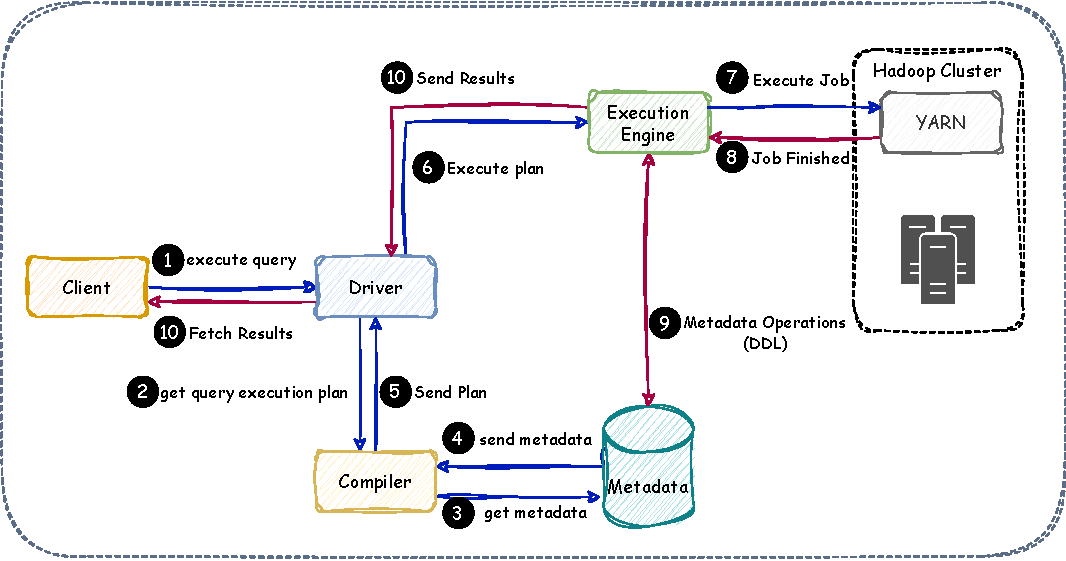
\includegraphics[width=\textwidth,height=\textheight,keepaspectratio]{./Figures/chapter-03/Hive_Query_Flow.pdf}
	\caption{Hive Job execution flow}
\end{figure}


	% \begin{itemize}
	% 	\item Receive SQL Query.
	% 	\begin{itemize}
	% 		\item Parse HiveQL.
	% 		\item Make optimization.
	% 		\item Plan execution.
	% 		\item Submit job(s) to the cluster.
	% 		\item Monitor the progress.
	% 		\item Process the data in MapReduce or Spark.
	% 		\item Store the data in HDFS.
	% 	\end{itemize}
	% \end{itemize}
	\end{frame}


%%%%%%%%%%%%%%%%%%%%%%%%%%%%%%%%%%%%%%%%%%%%%%%%%%%%%%
%%%%%%%%%%%%%%%%%%%%%%%%%%%%%%%%%%%%%%%%%%%%%%%%%%%%%%
\subsubsection{Hive Table Format}
%%%%%%%%%%%%%%%%%%%%%%%%%%%%%%%%%%%%%%%%%%%%%%%%%%%%%%
\begin{frame}{Hive Table Format}

	\begin{itemize}
		\item Hive was created to convert SQL statements into MapReduce jobs. \pause
		\item Mechanism needed for SQL to identify files and metadata. \pause
		\item Hive was a breakthrough, linking directories and files to tables. \pause
		\item HDFS directories map to database schemas and tables. \pause

	
	\end{itemize}
	\end{frame}
%%%%%%%%%%%%%%%%%%%%%%%%%%%%%%%%%%%%%%%%%%%%%%%%%%%%%%
\begin{frame}{Hive Table Format | continued}

	\begin{itemize}
		\item This was a breakthrough as it enabled working directly with the object store (i.e., HDFS) as the primary database storage, eliminating the need for custom file formats. \pause
		\item It also introduced flexibility in adding more file input formats (open formats), such as CSV, ORC, AVRO, Parquet, etc. Any processing that can be done with Map-Reduce can be applied to Hive. \pause
        \item Hive uses metastore/metadata to map raw HDFS data to named columns and types. \pause
		\item Each Hive table belongs to a specific database. \pause
	
	\end{itemize}
	\end{frame}
%%%%%%%%%%%%%%%%%%%%%%%%%%%%%%%%%%%%%%%%%%%%%%%%%%%%%%
\begin{frame}{Technical components in a data lake}
	\begin{minipage}{\textwidth}
		\begin{tikzpicture}
		  % Place image at the left side
		  \node[anchor=west] (image) at (0,0) {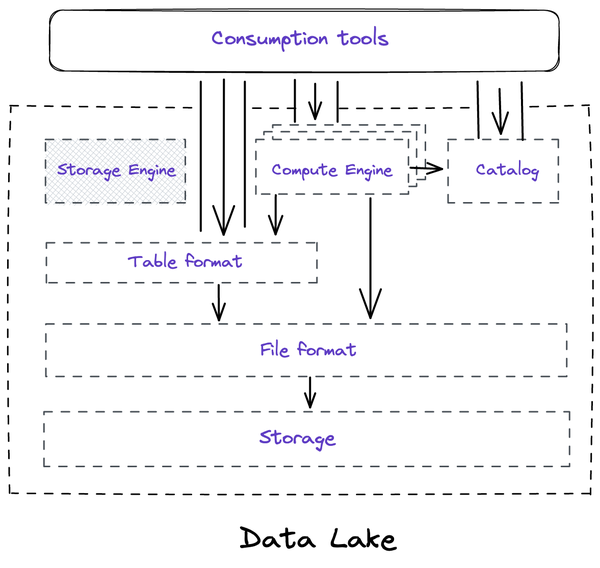
\includegraphics[width=\textwidth,height=.75\textheight,keepaspectratio]{./Figures/chapter-03/datalake_table_format.png}};
		  % Place text and arrow
		  \draw[<-, thick] (image) -- ++(4,1) node[right, align=left,font=\small, text=gray] {Apache Iceberg: The Definitive Guide: \\Data Lakehouse Functionality,\\ Performance, and Scalability\\ on the Data Lake\\ PUBLISHED BY:
		  O'Reilly Media, Inc.};
		\end{tikzpicture}
		\captionof{figure}{Technical components in a data lake}
	\end{minipage}
\end{frame}
%%%%%%%%%%%%%%%%%%%%%%%%%%%%%%%%%%%%%%%%%%%%%%%%%%%%%%
\begin{frame}{Hive Table Format | Example of Text File}

	\begin{itemize}
		\item Each Hive table links to a folder, usually on HDFS. \pause
		\item This folder contains one or more text files. \pause
		% \item Basics of Hive's default text format:
		% \begin{itemize}
		%   \item One record by line (\textbackslash n separator).
		%   \item Columns are split by Control-A (\textasciicircum A).
		%   \item Complex types use Control-B (\textasciicircum B).
		%   \item Map keys and values use Control-C (\textasciicircum C).
		% \end{itemize}
		% \item You can change these settings when making a new table.
	  \end{itemize}
	
	\end{frame}
%%%%%%%%%%%%%%%%%%%%%%%%%%%%%%%%%%%%%%%%%%%%%%%%%%%%%%
\begin{frame}{Text File vs. Binary File in Hive | High Level}
	\begin{table}[h!]
		\centering
		\resizebox{\textwidth}{!}{%
		%\begin{tabular}{|m{5cm}|m{6cm}|m{6cm}|}	    
			\begin{tabular}{|l|l|l|}
				\hline
				\rowcolor{Gray}
				Criteria & Text File & Binary File (e.g., ORC, Parquet) \\
				\hline
				Readability & Human-readable & Not human-readable \\
				\hline
				Debugging & Easier & Harder \\
				\hline
				Storage Size & Larger & More efficient \\
				\hline
				Speed & Slower & Faster \\
				\hline
				Delimiters & Basic (e.g., Control-A) & Complex types supported \\
				\hline
				Suitability & Small datasets & Large datasets \\
				\hline
			  \end{tabular}
	}
	\caption{Comparison between Text and Binary File Formats in Hive}	
  \end{table}
\end{frame}
%%%%%%%%%%%%%%%%%%%%%%%%%%%%%%%%%%%%%%%%%%%%%%%%%%%%%%
\begin{frame}{Why Binary Format is Faster than Text Format}
	\begin{table}[h!]
		\centering
		\resizebox{\textwidth}{!}{%
		%\begin{tabular}{|m{5cm}|m{6cm}|m{6cm}|}	    
		\begin{tabular}{|l|l|l|}
				\hline
				\rowcolor{Gray}
				Factor & Text File & Binary File \\
				\hline
				Parsing & Needs conversion & Directly readable \\
				\hline
				Memory & Less efficient & Efficient \\
				\hline
				Storage & Larger files & Smaller due to compression \\
				\hline
				Compression & Basic & Advanced algorithms \\
				\hline
				IO Operations & More reads/writes & Fewer reads/writes \\
				\hline
				Schema Evolution & Harder & Easier \\
				\hline
		\end{tabular}
	}
	\caption{Summary: Binary formats are generally more efficient in reading, writing, and storing data, making them faster for large datasets.}
  \end{table}
  \end{frame}
%%%%%%%%%%%%%%%%%%%%%%%%%%%%%%%%%%%%%%%%%%%%%%%%%%%%%%
\subsection{Hive Data Management}
\subsubsection{Hive Database}

%%%%%%%%%%%%%%%%%%%%%%%%%%%%%%%%%%%%%%%%%%%%%%%%%%%%%%
\begin{frame}[fragile]{Understanding Hive Database}
	\begin{itemize}
	  \item \textbf{What is Hive Database?}
		\begin{itemize}
		  \item A namespace for tables.
		  \item Helps in organizing data in Hive.
		  \item Namespaces function to avoid naming conflicts for tables, views, partitions, columns, and so on.  Databases can also be used to enforce security for a user or group of users.
		\end{itemize}
	  
	  \item \textbf{Table Organization}
		\begin{itemize}
		  \item Groups related tables under a single database.
		  \item Simplifies data management.
		  \item Homogeneous units of data which have the same schema.
		\end{itemize}
		
	\end{itemize}
  \end{frame}
%%%%%%%%%%%%%%%%%%%%%%%%%%%%%%%%%%%%%%%%%%%%%%%%%%%%%%
\begin{frame}[fragile]{Hive Warehouse Structure}
%\vspace{-0.5cm}
\begin{figure}

\includegraphics[width=\textwidth,height=.75\textheight]{./Figures/chapter-03/mermaid-diagram-hive_db.png}

\caption{Hive database structure}	
\end{figure}
\end{frame}
%%%%%%%%%%%%%%%%%%%%%%%%%%%%%%%%%%%%%%%%%%%%%%%%%%%%%%
\begin{frame}[fragile]{Hive Warehouse Structure | continued}

%\vspace{.6cm}
\begin{figure}
	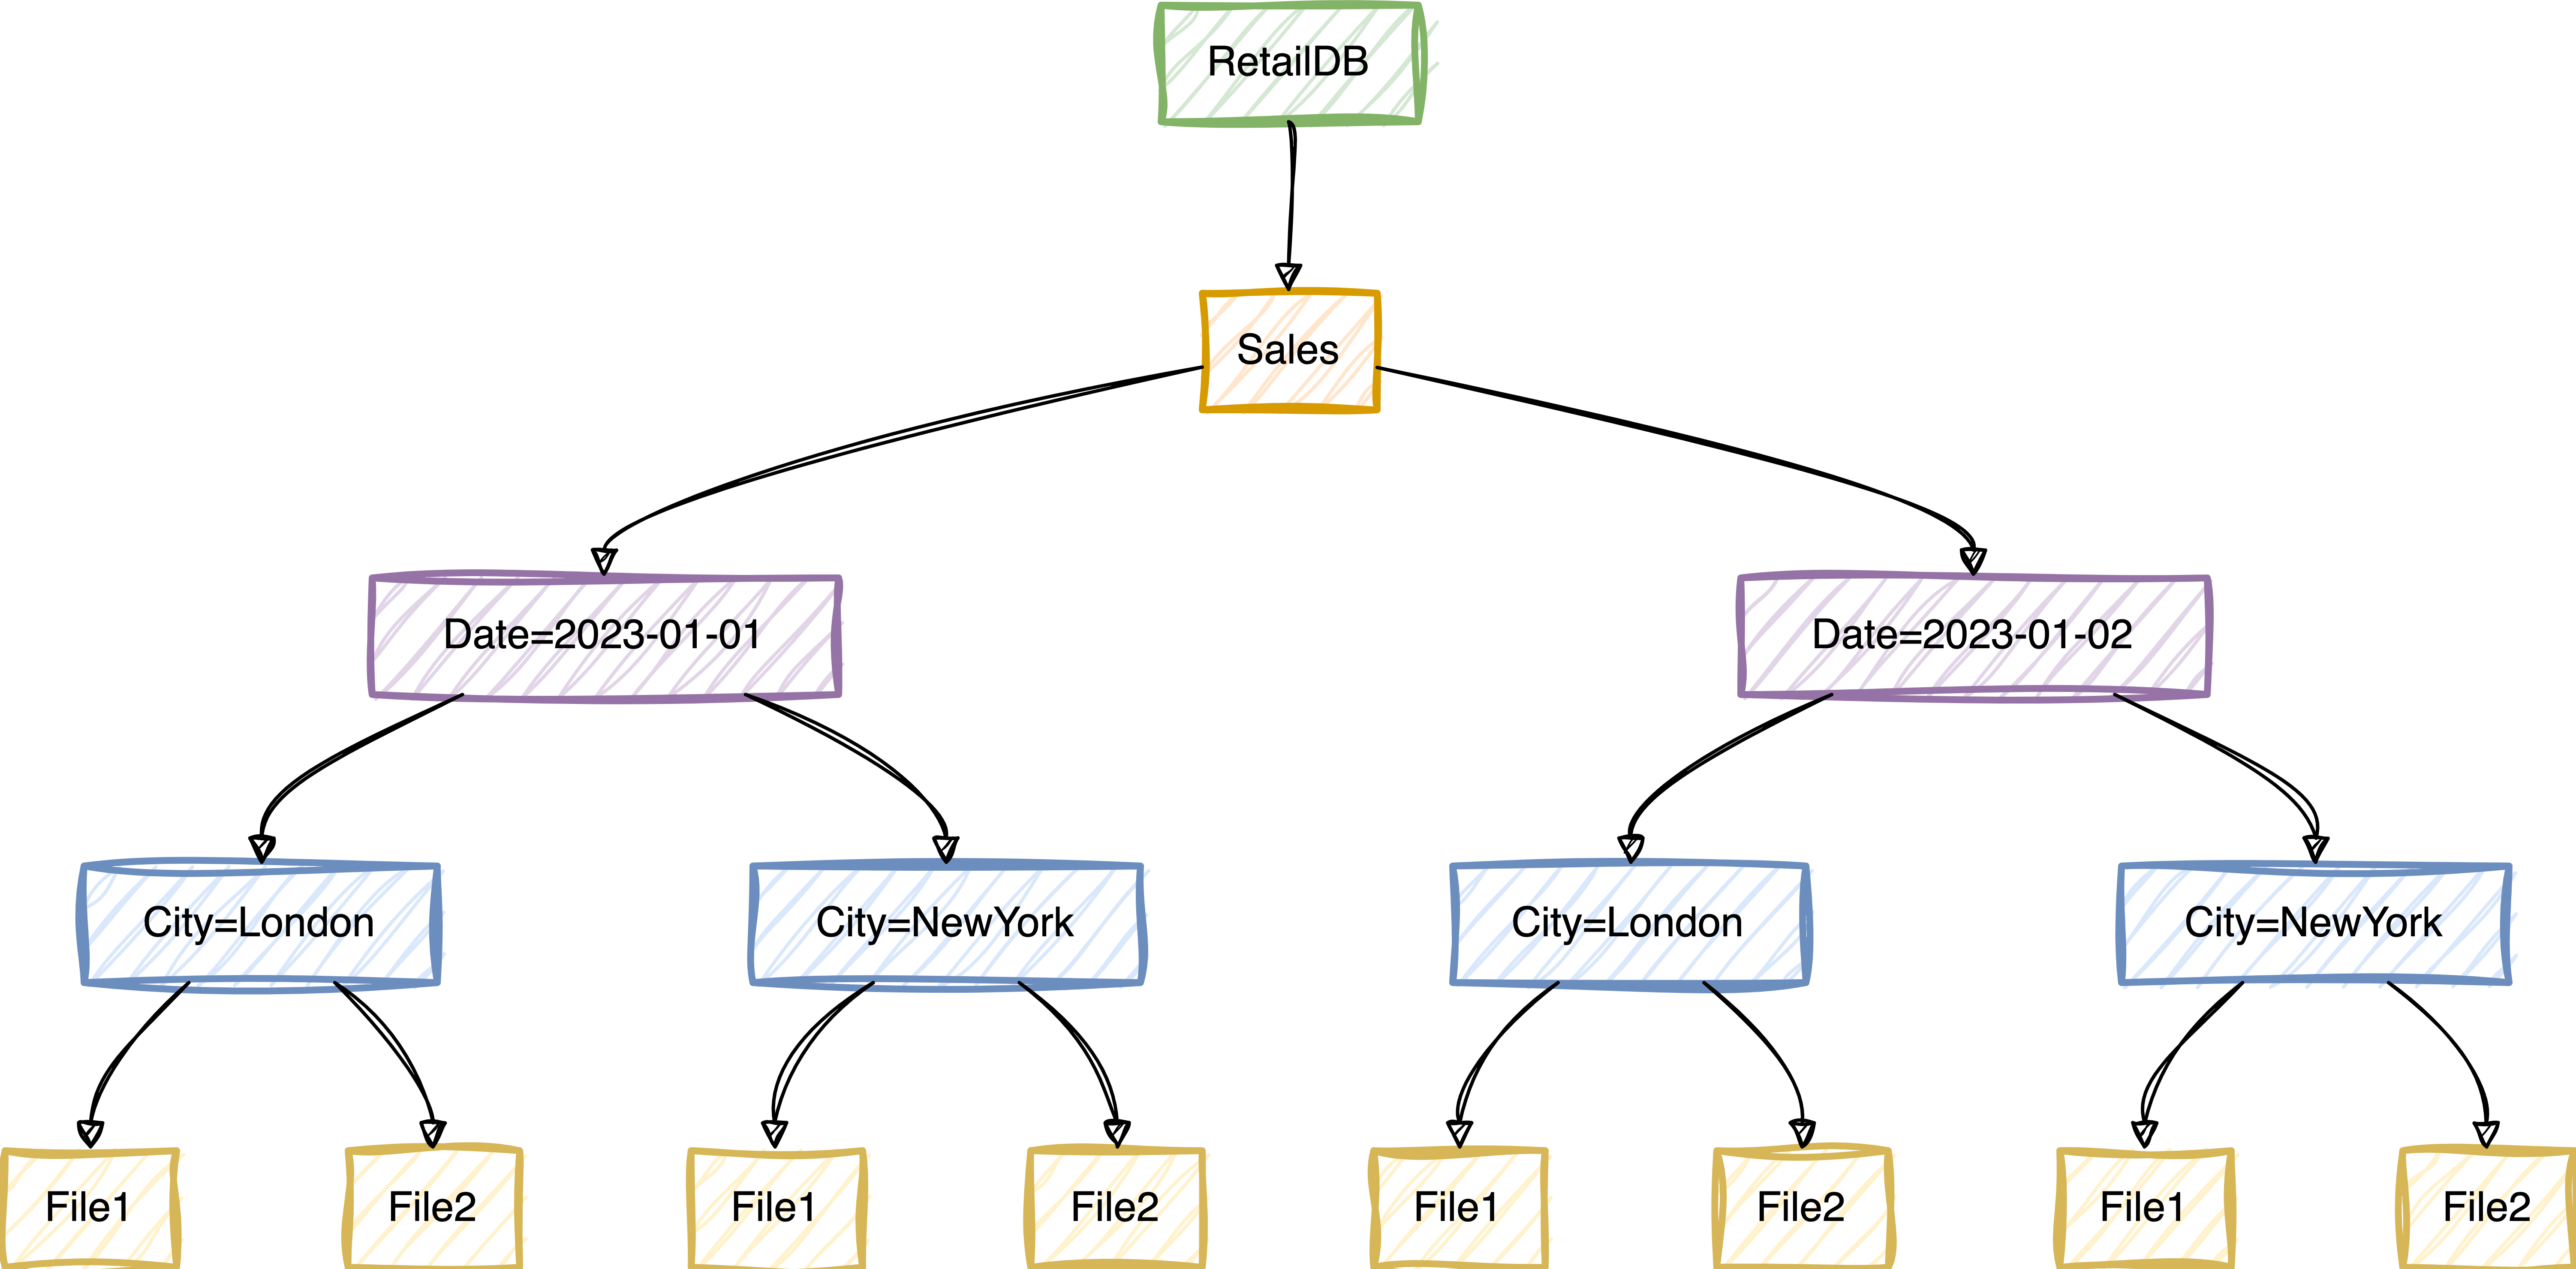
\includegraphics[width=\textwidth,height=.65\textheight]{./Figures/chapter-03/mermaid-diagram-retail_db.png}
	
	\caption{Hive database structure | Retail DB Example}	
\end{figure}
\end{frame}
%%%%%%%%%%%%%%%%%%%%%%%%%%%%%%%%%%%%%%%%%%%%%%%%%%%%%%
\begin{frame}[fragile]{Hive Warehouse Structure | continued}

%\vspace{.6cm}
	\begin{figure}
	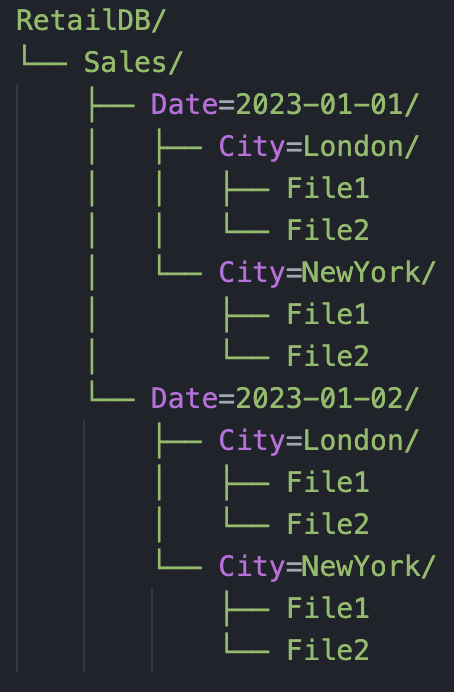
\includegraphics[width=\textwidth,height=.65\textheight,keepaspectratio]{./Figures/chapter-03/Screenshot_retail_db.png}
		
	\caption{Hive database structure | Retail DB HDFS Structure}	
	\end{figure}
	\end{frame}

%%%%%%%%%%%%%%%%%%%%%%%%%%%%%%%%%%%%%%%%%%%%%%%%%%%%%
\begin{frame}[fragile]{Creating Database in Hive}

\begin{lstlisting}[caption={Create Database command in Hive},language=SQL]
CREATE [REMOTE] (DATABASE|SCHEMA) [IF NOT EXISTS] database_name
[COMMENT database_comment]
[LOCATION hdfs_path]
[MANAGEDLOCATION hdfs_path]
[WITH DBPROPERTIES (property_name=property_value, ...)];  
\end{lstlisting}	
\begin{lstlisting}[caption={Create Database Example},language=SQL]
CREATE DATABASE hrDB;
USE hrDB;
\end{lstlisting}		

\end{frame}  

%%%%%%%%%%%%%%%%%%%%%%%%%%%%%%%%%%%%%%%%%%%%%%%%%%%%%
\begin{frame}[fragile]{Drop Database in Hive}

\begin{lstlisting}[caption={Drop Database command in Hive},language=SQL]
DROP (DATABASE|SCHEMA) [IF EXISTS] database_name [RESTRICT|CASCADE];
\end{lstlisting}		
	
\end{frame} 

%%%%%%%%%%%%%%%%%%%%%%%%%%%%%%%%%%%%%%%%%%%%%%%%%%%%%
\begin{frame}[fragile]{Alter Database in Hive}

\begin{lstlisting}[caption={Alter Database command in Hive},language=SQL]
ALTER (DATABASE|SCHEMA) database_name 
SET DBPROPERTIES (property_name=property_value, ...);
\end{lstlisting}		
\begin{lstlisting}[caption={Alter Database Example},language=SQL]
ALTER (DATABASE|SCHEMA) database_name SET LOCATION hdfs_path;
\end{lstlisting}		
\end{frame} 

%%%%%%%%%%%%%%%%%%%%%%%%%%%%%%%%%%%%%%%%%%%%%%%%%%%%%
\begin{frame}[fragile]{Use Database in Hive}

\begin{lstlisting}[caption={Alter Database command in Hive},language=SQL]
USE database_name;
USE DEFAULT;
\end{lstlisting}		
\end{frame} 
%%%%%%%%%%%%%%%%%%%%%%%%%%%%%%%%%%%%%%%%%%%%%%%%%%%%%%

\begin{frame}[fragile]{Hive Schema vs. Database}		  
	\begin{itemize}
	  \item In Hive, the terms 'schema' and 'database' are interchangeable.
	  \item Both serve as a namespace for tables.
	\end{itemize}	
	\begin{tcolorbox}[colback=white, colframe=black, title=\scriptsize From Hive Documentation]
		\small \color{darkgray}{\textit{%
		"The uses of SCHEMA and DATABASE are interchangeable – they mean the same thing. CREATE DATABASE was added in Hive 0.6 (HIVE-675). The WITH DBPROPERTIES clause was added in Hive 0.7 (HIVE-1836)."
		}}
	  \end{tcolorbox}
	
\end{frame}


%%%%%%%%%%%%%%%%%%%%%%%%%%%%%%%%%%%%%%%%%%%%%%%%%%%%%%
\subsubsection{Hive Tables}
%%%%%%%%%%%%%%%%%%%%%%%%%%%%%%%%%%%%%%%%%%%%%%%%%%%%%%
\begin{frame}[fragile]{Creating Tables in Hive}
\vspace{-.2cm}
\begin{lstlisting}[caption={Create Table Commands},language=SQL]
CREATE [TEMPORARY] [EXTERNAL] TABLE [IF NOT EXISTS] [db_name.]table_name
[(col_name data_type [column_constraint_specification] [COMMENT col_comment], ... [constraint_specification])]
[COMMENT table_comment]
[PARTITIONED BY (col_name data_type [COMMENT col_comment], ...)]
[CLUSTERED BY (col_name, col_name, ...) [SORTED BY (col_name [ASC|DESC], ...)] INTO num_buckets BUCKETS]
[SKEWED BY (col_name, col_name, ...)
ON ((col_value, col_value, ...), (col_value, col_value, ...), ...)
[STORED AS DIRECTORIES]
[[ROW FORMAT row_format] 
[STORED AS file_format]
|STORED BY 'storage.handler.class.name' [WITH SERDEPROPERTIES (...)]]
[LOCATION hdfs_path]
[TBLPROPERTIES (property_name=property_value, ...)]
[AS select_statement];
\end{lstlisting}

\end{frame}

%%%%%%%%%%%%%%%%%%%%%%%%%%%%%%%%%%%%%%%%%%%%%%%%%%%%%%
\begin{frame}{CREATE TABLE in Hive | continued}
	\begin{tcolorbox}[colback=white,colframe=black,title= Part 1: Table Creation Basics]
		\small
		\begin{itemize}
			\item \texttt{CREATE [TEMPORARY] [EXTERNAL] TABLE [IF NOT EXISTS] [db\_name.]table\_name}
			\begin{itemize}
			  \item \texttt{TEMPORARY}: Creates a temporary table.
			  \item \texttt{EXTERNAL}: Defines the table as an external table.
			  \item \texttt{IF NOT EXISTS}: Only creates if the table does not exist.
			  \item \texttt{db\_name.table\_name}: Specifies database and table name.
			\end{itemize}
		  \end{itemize}
	\end{tcolorbox}

  \end{frame}
%%%%%%%%%%%%%%%%%%%%%%%%%%%%%%%%%%%%%%%%%%%%%%%%%%%%%%
  \begin{frame}{CREATE TABLE in Hive | continued}
	\begin{tcolorbox}[colback=white,colframe=black,title= Part 2: Column Definitions]
		\small
		\begin{itemize}
		\item \texttt{[(col\_name data\_type [COMMENT col\_comment], ...)]}
			\begin{itemize}
				\item Define the columns and their data types.
				\item Optional comment for each column.
			\end{itemize}
		\end{itemize}
	\end{tcolorbox}
\end{frame}
%%%%%%%%%%%%%%%%%%%%%%%%%%%%%%%%%%%%%%%%%%%%%%%%%%%%%%
\begin{frame}{CREATE TABLE in Hive | continued}
	\begin{tcolorbox}[colback=white,colframe=black,title= Part 2: Column Definitions (data_type)]
		\small	
			\begin{itemize}	
				\vspace{-0.2cm}\item \textbf{Primitive Type}: Basic data types like INT, BIGINT, BOOLEAN, FLOAT, DOUBLE, STRING, TIMESTAMP, DECIMAL, DATE, etc.
				\vspace{-0.2cm}\item \textbf{Array Type}: Ordered sequences of the same type, e.g., ARRAY<INT>.			
				\vspace{-0.2cm}\item \textbf{Map Type}: Key-value pairs, e.g., MAP<STRING, INT>.				
				\vspace{-0.2cm}\item \textbf{Struct Type}: Collection of named fields that can be different types, e.g., STRUCT<field1:STRING, field2:INT>.				
				\vspace{-0.2cm}\item \textbf{Union Type}: Can be any of the specified types, e.g., UNIONTYPE<STRING, INT>.		  
			\end{itemize}
	\end{tcolorbox}
\end{frame}
%%%%%%%%%%%%%%%%%%%%%%%%%%%%%%%%%%%%%%%%%%%%%%%%%%%%%%
\begin{frame}{CREATE TABLE in Hive | continued}
	\begin{tcolorbox}[colback=white,colframe=black,title= Part 3: Row Format and SerDe in Hive]
		\small
	\begin{itemize}
	  \item \texttt{[ROW FORMAT row\_format]}
	  \begin{itemize}
		\item Specifies the row format (e.g., delimited, sequence file, etc.)
		\item Native SerDe is used if ROW FORMAT is not specified or ROW FORMAT DELIMITED is specified.
		\item Use SERDE clause for custom SerDe.
	  \end{itemize}
	\end{itemize}
	\end{tcolorbox}
  \end{frame}
%%%%%%%%%%%%%%%%%%%%%%%%%%%%%%%%%%%%%%%%%%%%%%%%%%%%%%
\begin{frame}[fragile]{CREATE TABLE in Hive | continued}


\textbf{RegEx Example}
\begin{lstlisting}[caption={RegEx Example},language=SQL]
ROW FORMAT SERDE 'org.apache.hadoop.hive.serde2.RegexSerDe'
WITH SERDEPROPERTIES ("input.regex" = "<regex>")
STORED AS TEXTFILE;
\end{lstlisting}
  
\textbf{CSV/TSV Example}
\begin{lstlisting}[caption={CSV/TSV Example},language=SQL]
ROW FORMAT SERDE 'org.apache.hadoop.hive.serde2.OpenCSVSerde'
WITH SERDEPROPERTIES ("separatorChar" = "\t","quoteChar" = "'", "escapeChar" = "\\")
STORED AS TEXTFILE;
\end{verbatim}
\end{lstlisting}	  


  \end{frame}
  
%%%%%%%%%%%%%%%%%%%%%%%%%%%%%%%%%%%%%%%%%%%%%%%%%%%%%%
  \begin{frame}{CREATE TABLE in Hive | continued}
	\begin{tcolorbox}[colback=white,colframe=black,title= Part 4: File Format and Storage Handler]
		\small
	\begin{itemize}
	  \item \texttt{[STORED AS file\_format | STORED BY 'storage.handler.class.name']}
	  \begin{itemize}
		\item Specifies the file format (e.g., TEXTFILE, PARQUET, SEQUENCEFILE, ORC, AVRO, JSONFILE etc.).
		\item Custom storage handler (e.g., INPUTFORMAT input_format_classname OUTPUTFORMAT output_format_classname)
	  \end{itemize}
	\end{itemize}
	\end{tcolorbox}
  \end{frame}
%%%%%%%%%%%%%%%%%%%%%%%%%%%%%%%%%%%%%%%%%%%%%%%%%%%%%%
  \begin{frame}{CREATE TABLE in Hive | continued}
	\begin{tcolorbox}[colback=white,colframe=black,title= Part 5: Table Partitions]
		\small
	\begin{itemize}
	  \item \texttt{[PARTITIONED BY (col\_name data\_type [COMMENT col\_comment], ...)]}
	  \begin{itemize}
		\item Specifies columns to be used for partitioning.
		\vspace{-0.2cm}\item Partitioned tables can be created using the \textcolor{blue}{\textbf{\texttt{PARTITIONED BY}}} clause.
		\vspace{-0.2cm}\item A table can have one or more partition keys, and a separate data directory is created for each distinct value combination in the partition columns.
		\vspace{-0.2cm}\item Partitioning enables efficient data filtering.
		
	  \end{itemize}
	\end{itemize}
	\end{tcolorbox}
  \end{frame}
%%%%%%%%%%%%%%%%%%%%%%%%%%%%%%%%%%%%%%%%%%%%%%%%%%%%%%
  \begin{frame}[fragile]
	\frametitle{CREATE TABLE in Hive | continued}
	\begin{tcolorbox}[colback=white,colframe=black,title= Part 5: Table Partitions]
		\small
\begin{lstlisting}[caption={Create Partitioned Table},language=SQL]
CREATE TABLE sales (
product_id INT,
order_date STRING,
amount DOUBLE
)
PARTITIONED BY (year INT, region STRING)
ROW FORMAT DELIMITED
FIELDS TERMINATED BY ','
STORED AS TEXTFILE;
\end{lstlisting}
\end{tcolorbox}

\end{frame}
%%%%%%%%%%%%%%%%%%%%%%%%%%%%%%%%%%%%%%%%%%%%%%%%%%%%%%	
	\begin{frame}[fragile]
	\frametitle{CREATE TABLE in Hive | continued}
	\begin{tcolorbox}[colback=white,colframe=black,title= Part 5: Table Partitions]
		\small

	\begin{itemize}
	\item \textbf{Table:} sales
	\item \textbf{Columns:} product_id, order_date, amount
	\item \textbf{Partition Columns:} year, region
	\end{itemize}
	This table stores sales records. Each record includes the \textit{product\_id}, \textit{order\_date}, and \textit{amount} of the sale.
\end{tcolorbox}
	
\end{frame}
%%%%%%%%%%%%%%%%%%%%%%%%%%%%%%%%%%%%%%%%%%%%%%%%%%%%%%
\begin{frame}[fragile]
\frametitle{CREATE TABLE in Hive | continued}
\vspace{-0.5cm}\begin{tcolorbox}[colback=white,colframe=black,title= Part 5: Table Partitions]
\small
\vspace{-0.2cm}
\begin{figure}
	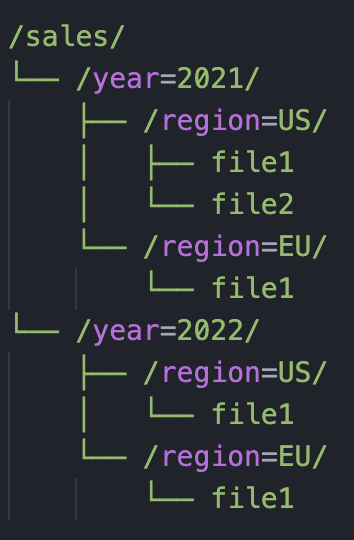
\includegraphics[width=\textwidth,height=.6\textheight,keepaspectratio]{./Figures/chapter-03/Screenshot_partitioned_example.png}
	\caption{Hive database structure | Retail DB HDFS Structure}	
	\end{figure}	
\end{tcolorbox}
	
\end{frame}

% %%%%%%%%%%%%%%%%%%%%%%%%%%%%%%%%%%%%%%%%%%%%%%%%%%%%%%
% \begin{frame}[fragile]
% \frametitle{CREATE TABLE in Hive | continued}
% \vspace{-0.5cm}\begin{tcolorbox}[colback=white,colframe=black,title= Part 5: Table Partitions]
% \small
% \vspace{-0.2cm}
% \begin{lstlisting}[caption={Explain Plan Command for Non-Partitioned Table }]
% /sales/
% |___ /year=2021/
%     |___ /region=US/
%     |       |___ file1
%     |       |___ file2
%     |___ /region=EU/
%             |___ file1
% |___ /year=2022/
%     |___ /region=US/
%     |       |___ file1
%     |___ /region=EU/
%             |___ file1
% \end{lstlisting}
% \end{tcolorbox}	
%\end{frame}
%%%%%%%%%%%%%%%%%%%%%%%%%%%%%%%%%%%%%%%%%%%%%%%%%%%%%%
\begin{frame}[fragile]
\frametitle{CREATE TABLE in Hive | continued}
\begin{tcolorbox}[colback=white,colframe=black,title= Part 5: Table Partitions]
\small
\begin{lstlisting}[caption={Simple sql statement for sales table filters on year and region},language=SQL]
SELECT * FROM sales WHERE year=2021 AND region='US';
\end{lstlisting}
\vspace{-0.5cm}
  \begin{table}[h!]
	\centering
	\resizebox{\textwidth}{!}{%
		\begin{tabular}{|p{6cm}|p{6cm}|}
			\hline
			\rowcolor{Gray}
			Non-Partitioned Table & Partitioned Table \\
			\hline
			Step 1: Full table scan & Step 1: Identify partitions (\texttt{year=2021, region='US'}) \\
			\hline
			Step 2: Apply \texttt{WHERE} filters (\texttt{year=2021 AND region='US'}) & Step 2: Scan only those partitions \\
			\hline
		  \end{tabular}
		}
\caption{Comparison: Non-Partitioned vs Partitioned Table.}
\end{table}

\end{tcolorbox}

\end{frame}
%%%%%%%%%%%%%%%%%%%%%%%%%%%%%%%%%%%%%%%%%%%%%%%%%%%%%%
\begin{frame}[fragile]
	\frametitle{CREATE TABLE in Hive | continued}
	\vspace{-0.6cm}
	\begin{tcolorbox}[colback=white,colframe=black,title= Part 5: Table Partitions]
	\small
	\vspace{-0.3cm}
\begin{lstlisting}[caption={Explain Plan Command for Non-Partitioned Table },language=SQL]
EXPLAIN SELECT * FROM sales_non_partitioned WHERE year=2021 AND region='US';
\end{lstlisting}
\vspace{-0.5cm}
\begin{lstlisting}[caption={Explain Plan Command for Non-Partitioned Table },language=SQL]
STAGE PLANS:
Stage: Stage-1
  Map Reduce
    Map Operator Tree:
        TableScan
          alias: sales
          Filter Operator
            predicate: (year = 2021 and region = 'US')
 
\end{lstlisting}
\end{tcolorbox}
	
\end{frame}
%%%%%%%%%%%%%%%%%%%%%%%%%%%%%%%%%%%%%%%%%%%%%%%%%%%%%%
\begin{frame}[fragile]
	\frametitle{CREATE TABLE in Hive | continued}
	\vspace{-0.6cm}
	\begin{tcolorbox}[colback=white,colframe=black,title= Part 5: Table Partitions]
	\small
	\vspace{-0.3cm}
\begin{lstlisting}[caption={Explain Plan Command for Partitioned Table },language=SQL]
EXPLAIN SELECT * FROM sales_partitioned WHERE year=2021 AND region='US';
\end{lstlisting}
	\vspace{-0.5cm}
\begin{lstlisting}[caption={Explain Plan Command for Partitioned Table },language=SQL]
    STAGE PLANS:
      Stage: Stage-1
        Map Reduce
          Map Operator Tree:
              TableScan
                alias: sales_partitioned
                Filter Operator
                  predicate: (year = 2021 and region = 'US')
          Partition Pruning: (year = 2021 and region = 'US')
\end{lstlisting}
\end{tcolorbox}
	
\end{frame}
%%%%%%%%%%%%%%%%%%%%%%%%%%%%%%%%%%%%%%%%%%%%%%%%%%%%%%
\begin{frame}[fragile]
	\frametitle{CREATE TABLE in Hive | continued}
	\begin{tcolorbox}[colback=white,colframe=black,title= Part 5: Table Partitions]
\vspace{.5cm}
	\begin{table}[h!]
		\centering
		\resizebox{\textwidth}{!}{%
		\begin{tabular}{|p{4cm}|p{5cm}|p{5cm}|}	
			\hline
			\rowcolor{Gray}
			Aspect & Non-Partitioned & Partitioned \\
			\hline
			Full Table Scan & Yes & No \\
			Partition Pruning & N/A & Yes \\
			I/O Cost & High & Low \\
			Time Complexity & More Time & Less Time \\
			Resource Utilization & High & Low \\
			\hline
	\end{tabular}
	}
\caption{Comparison: Non-Partitioned vs Partitioned Table.}
\end{table}
\end{tcolorbox}
	
\end{frame}

%%%%%%%%%%%%%%%%%%%%%%%%%%%%%%%%%%%%%%%%%%%%%%%%%%%%%%
%%%%%%%%%%%%%%%%%%%%%%%%%%%%%%%%%%%%%%%%%%%%%%%%%%%%%%
%%%%%%%%%%%%%%%%%%%%%%%%%%%%%%%%%%%%%%%%%%%%%%%%%%%%%%  
  \begin{frame}{CREATE TABLE in Hive | continued}
	\begin{tcolorbox}[colback=white,colframe=black,title= Part 6: Clustering and Sorting]
		\small
	\begin{itemize}
	  \item \texttt{[CLUSTERED BY (col\_name, ...) [SORTED BY (col\_name [ASC|DESC], ...)] INTO num\_buckets BUCKETS]}
	  \begin{itemize}
		\item Clustering and sorting options for better performance and to optimize data storage.
	  \end{itemize}
	\end{itemize}
	\end{tcolorbox}
  \end{frame}

%%%%%%%%%%%%%%%%%%%%%%%%%%%%%%%%%%%%%%%%%%%%%%%%%%%%%%	
\begin{frame}
\frametitle{CREATE TABLE in Hive | continued}
\begin{tcolorbox}[colback=white,colframe=black,title= Part 6: Clustering and Sorting | CLUSTERED BY]
	\small
	vspace{.2cm}
	\begin{table}[h!]
		\centering
		\resizebox{\textwidth}{!}{%
		\begin{tabular}{|p{2cm}|p{2cm}|p{2cm}|p{2cm}|}	
			\hline
			\rowcolor{Gray}
			ID & Name & Department & Salary \\
			\hline
			1 & John & HR & 5000 \\
			2 & Alice & Sales & 6000 \\
			3 & Bob & IT & 7000 \\
			4 & Carol & HR & 8000 \\
			5 & Dave & Sales & 9000 \\
			6 & Eve & IT & 4000 \\
			\hline
	  	\end{tabular}
		}
		\caption{Sample data for employee table}
	\end{table}
\end{tcolorbox}
\end{frame}
%%%%%%%%%%%%%%%%%%%%%%%%%%%%%%%%%%%%%%%%%%%%%%%%%%%%%%	
\begin{frame}[fragile]
\frametitle{CREATE TABLE in Hive | continued}	
\begin{tcolorbox}[colback=white,colframe=black,title= Part 6: Clustering and Sorting | CLUSTERED BY]
\small
\begin{lstlisting}[caption={Create CLUSTERED Table},language=SQL]
CREATE TABLE Employee (
  ID INT,
  Name STRING,
  Department STRING,
  Salary INT)
CLUSTERED BY (Department) INTO 3 BUCKETS;
\end{lstlisting}
\end{tcolorbox}
\end{frame}

%%%%%%%%%%%%%%%%%%%%%%%%%%%%%%%%%%%%%%%%%%%%%%%%%%%%%%	
% Slide 4: Bucket Distribution
\begin{frame}
\frametitle{CREATE TABLE in Hive | continued}
\begin{tcolorbox}[colback=white,colframe=black,title= Part 6: Clustering and Sorting | CLUSTERED BY]
	\begin{itemize}
		\item Bucket 1: Data for HR
		\item Bucket 2: Data for Sales
		\item Bucket 3: Data for IT
	\end{itemize}
\end{tcolorbox}
\end{frame}
%%%%%%%%%%%%%%%%%%%%%%%%%%%%%%%%%%%%%%%%%%%%%%%%%%%%%%		
\begin{frame}
	\frametitle{CREATE TABLE in Hive | continued}		
	\vspace{-0.5cm}
	\begin{tcolorbox}[colback=white,colframe=black,title= Part 6: Clustering and Sorting | CLUSTERED BY]
		\vspace{-0.2cm}
		\begin{figure}
			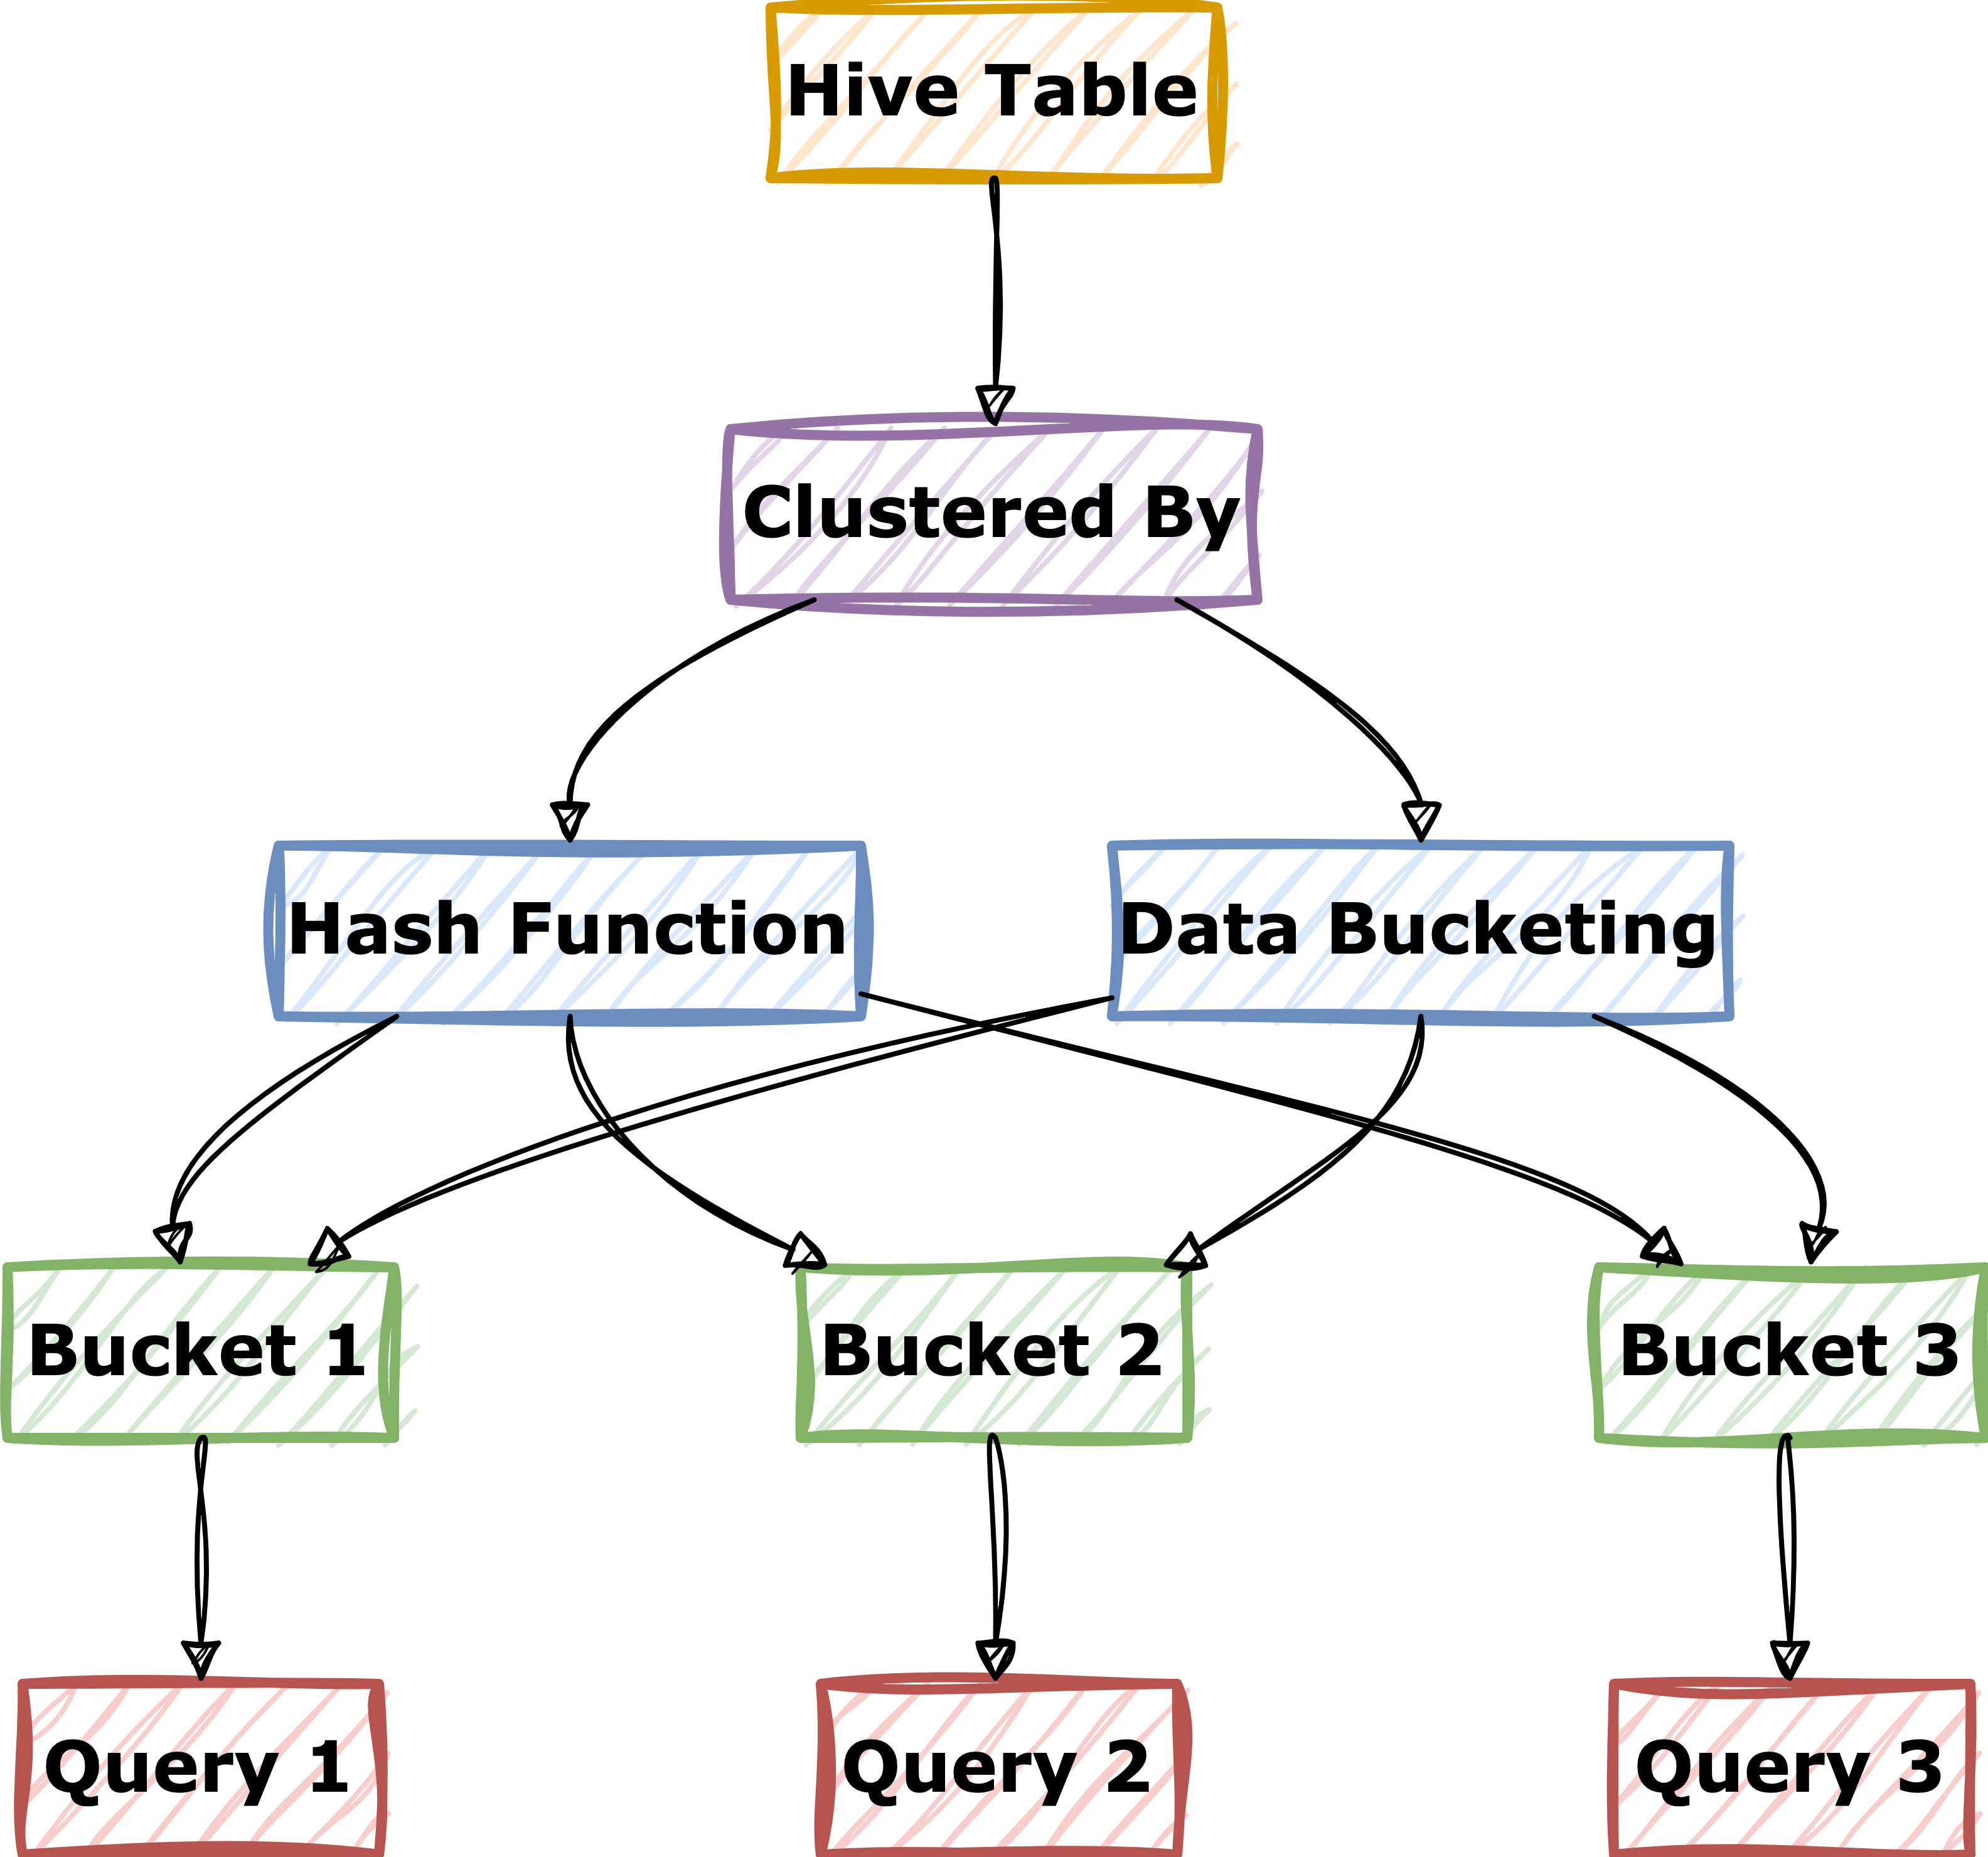
\includegraphics[width=\textwidth,height=.6\textheight,keepaspectratio]{./Figures/chapter-03/mermaid-diagram-hive_db_clustered_by.png}				
			\caption{Hive Table | Clustered by mechanism}	
		\end{figure}
	\end{tcolorbox}				
\end{frame}
%%%%%%%%%%%%%%%%%%%%%%%%%%%%%%%%%%%%%%%%%%%%%%%%%%%%%%		
\begin{frame}
	\frametitle{CREATE TABLE in Hive | continued}		
	\vspace{-0.5cm}
	\begin{tcolorbox}[colback=white,colframe=black,title= Part 6: Clustering and Sorting | CLUSTERED BY]
		\vspace{-0.2cm}
		\begin{figure}
			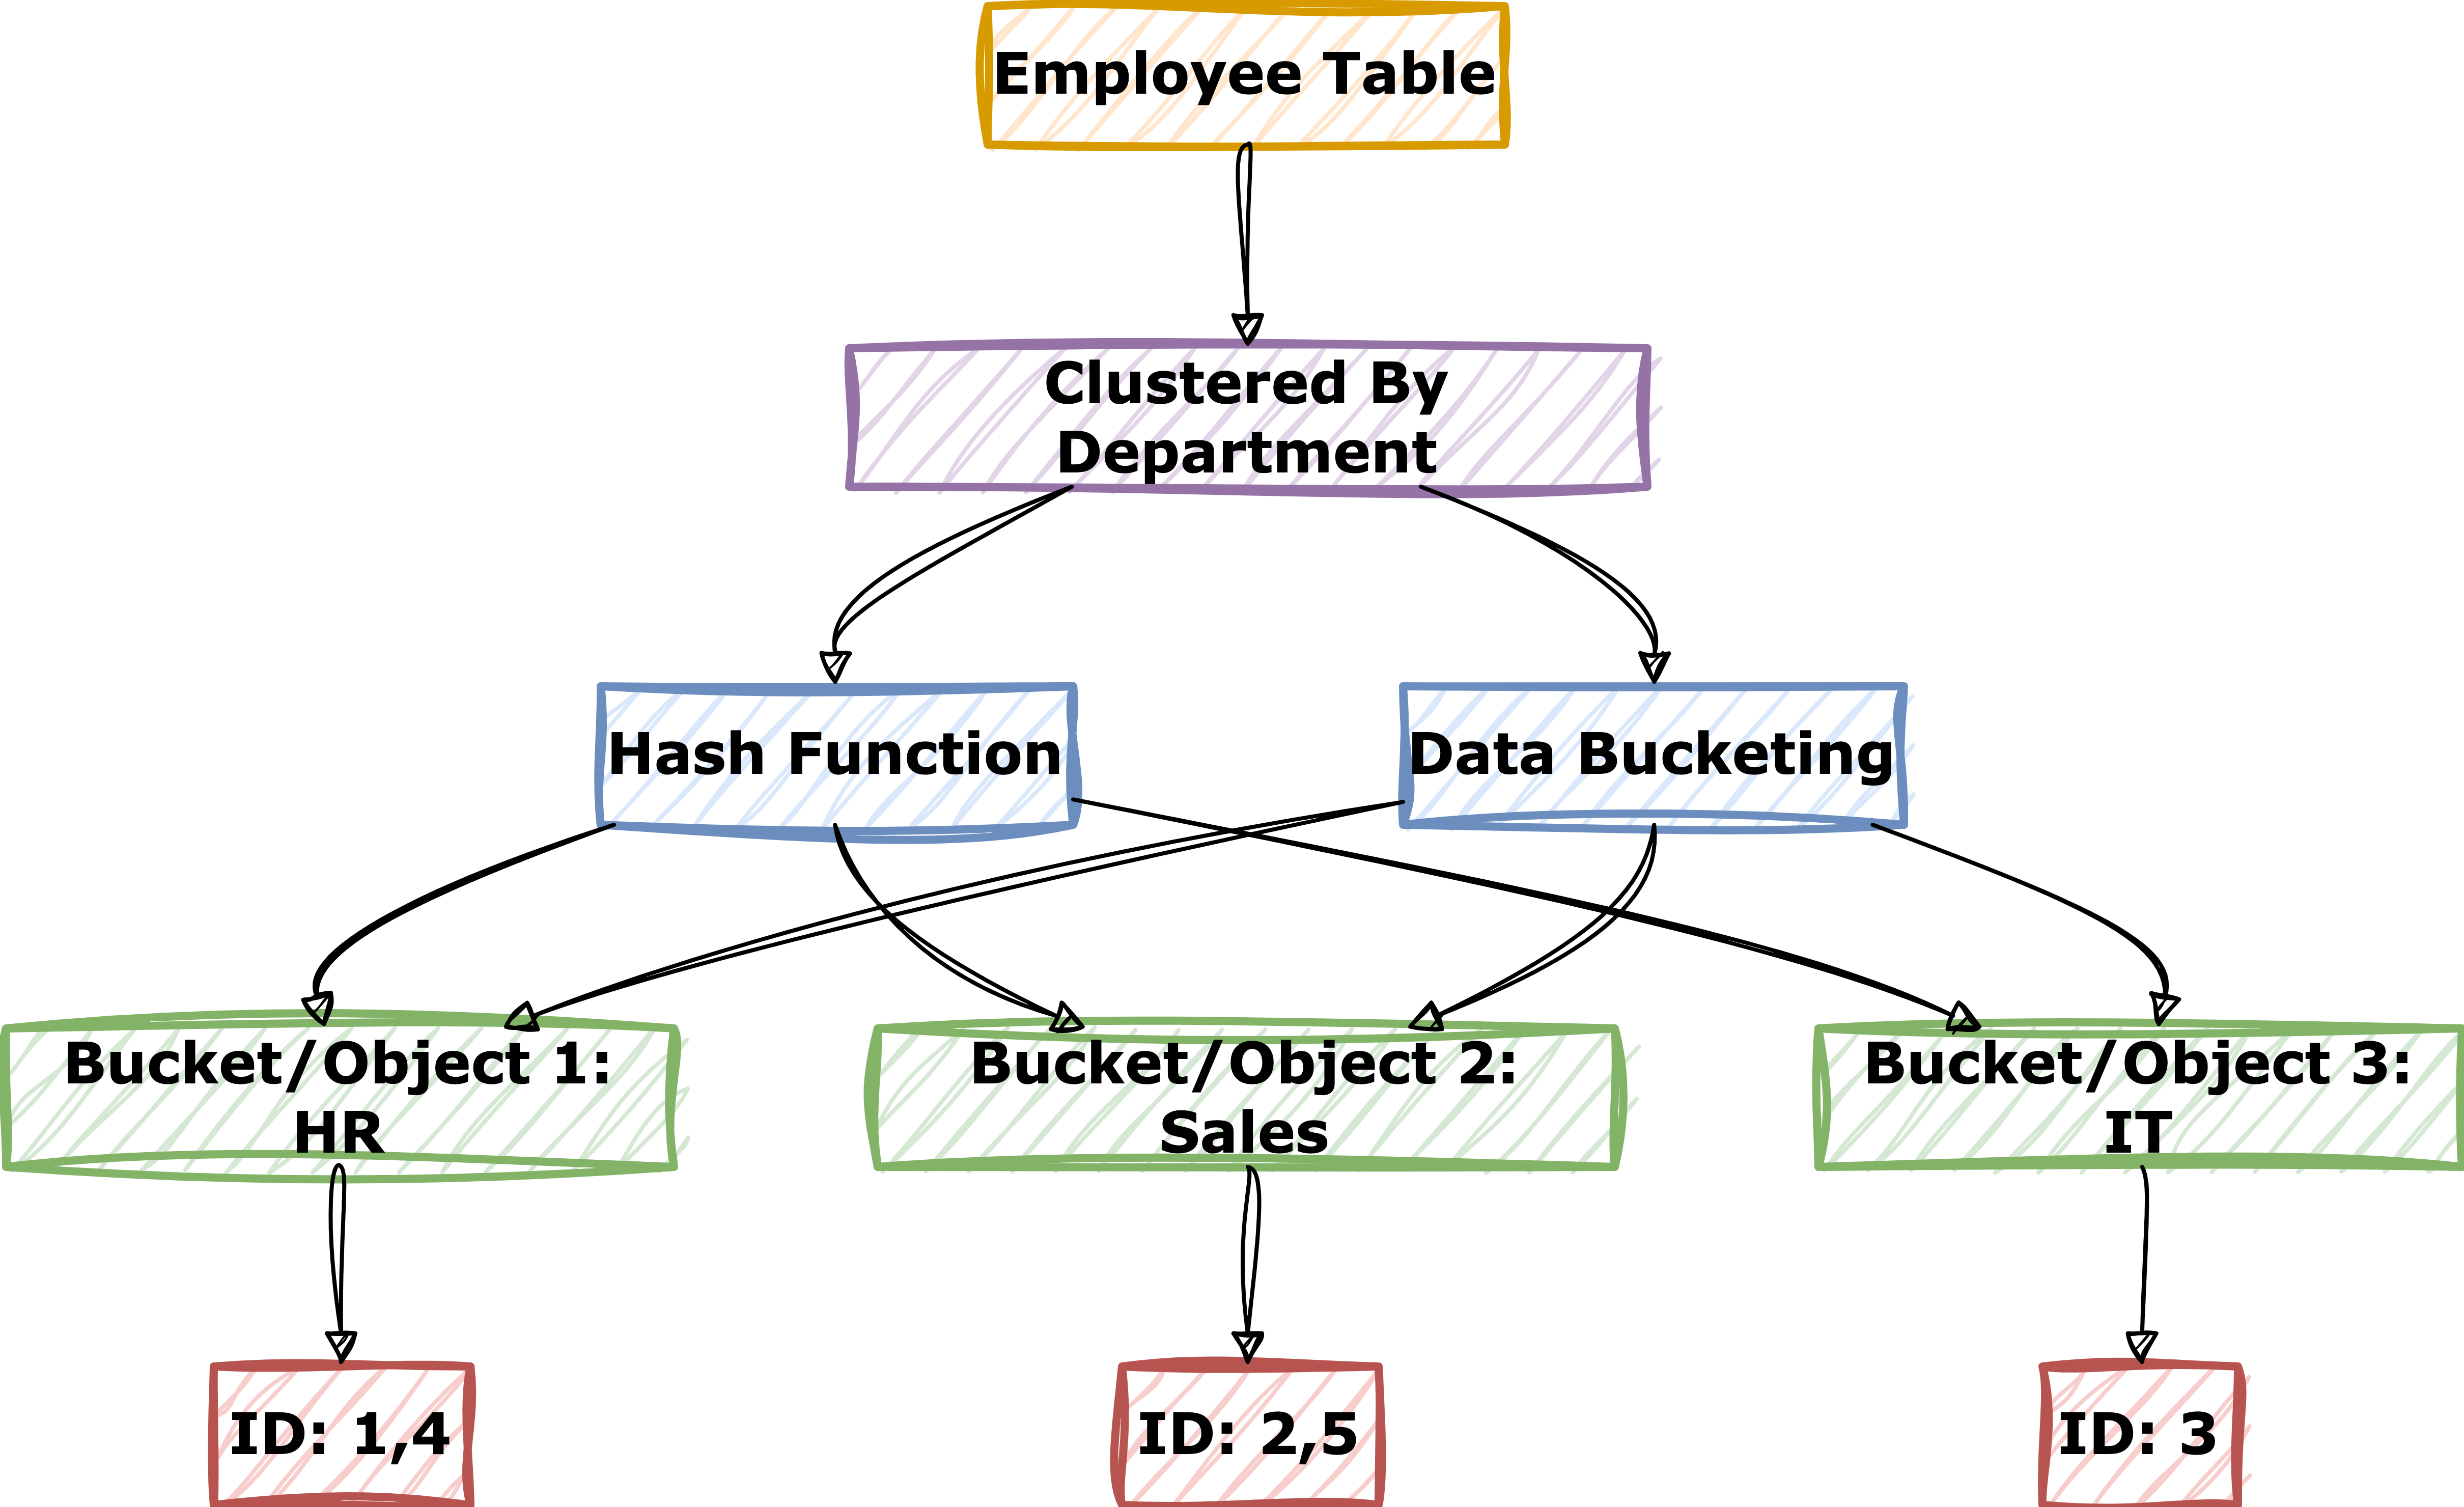
\includegraphics[width=\textwidth,height=.6\textheight,keepaspectratio]{./Figures/chapter-03/mermaid-diagram-hive_db_clustered_by_exp.png}				
			\caption{Hive Table | Clustered by mechanism example}	
		\end{figure}
	\end{tcolorbox}				
\end{frame}
%%%%%%%%%%%%%%%%%%%%%%%%%%%%%%%%%%%%%%%%%%%%%%%%%%%%%%		
\begin{frame}
	\frametitle{CREATE TABLE in Hive | continued}		
	\vspace{-0.5cm}
	\begin{tcolorbox}[colback=white,colframe=black,title= Part 6: Clustering and Sorting | CLUSTERED BY]
		\begin{figure}
			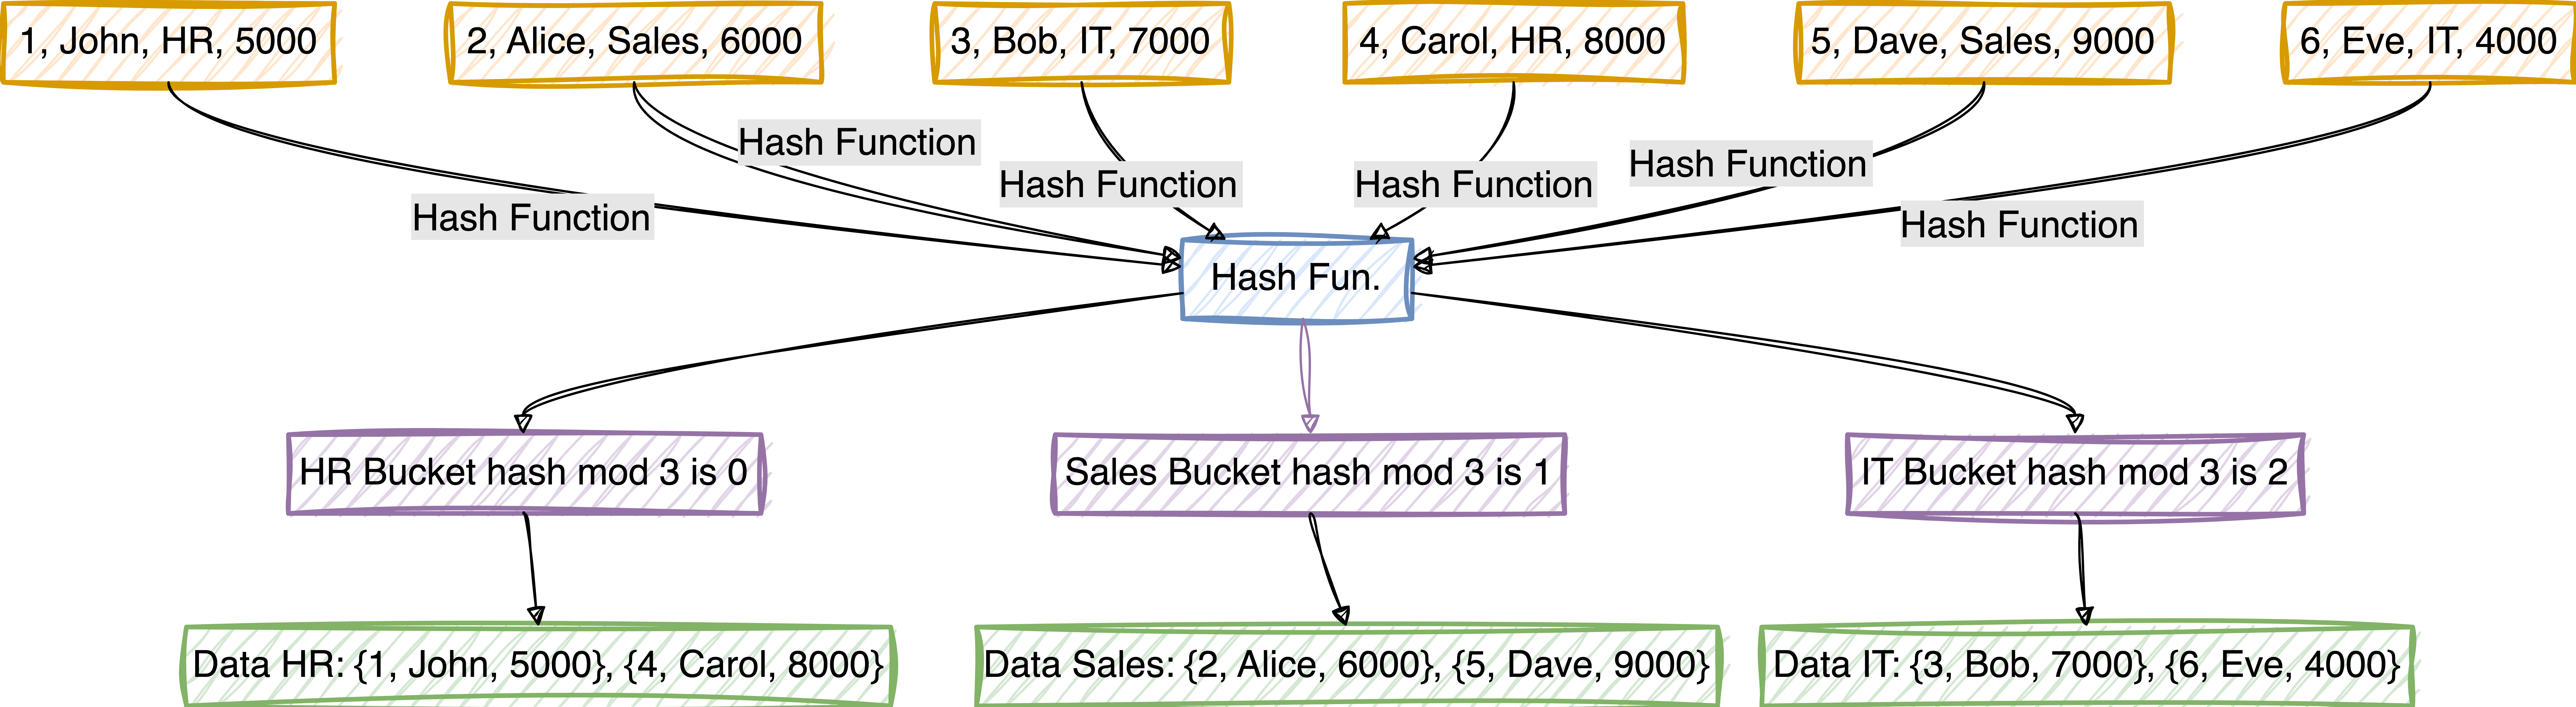
\includegraphics[width=\textwidth,height=1.2\textheight,keepaspectratio]{./Figures/chapter-03/mermaid-diagram-hive_db_clustered_by_exp_hash.png}				
			\caption{Hive Table | Clustered by mechanism example}	
		\end{figure}
	\end{tcolorbox}				
\end{frame}


%%%%%%%%%%%%%%%%%%%%%%%%%%%%%%%%%%%%%%%%%%%%%%%%%%%%%%	
\begin{frame}[fragile]
\frametitle{CREATE TABLE in Hive | continued}	
	\begin{tcolorbox}[colback=white,colframe=black,title= Part 6: Clustering and Sorting | CLUSTERED BY]
	\small
		\begin{lstlisting}[caption={Simple SQL statement},language=SQL]
		EXPLAIN SELECT * FROM Employee WHERE Department = 'HR';
		\end{lstlisting}
	\end{tcolorbox}
\end{frame}
%%%%%%%%%%%%%%%%%%%%%%%%%%%%%%%%%%%%%%%%%%%%%%%%%%%%%%	
\begin{frame}[fragile]
\frametitle{CREATE TABLE in Hive | continued}	
\vspace{-0.3cm}
\begin{tcolorbox}[colback=white,colframe=black,title= Part 6: Clustering and Sorting | CLUSTERED BY]
\small
\vspace{-0.3cm}
\begin{lstlisting}[caption={Simplified Explain Plan for Table Without CLUSTERED BY},style=my-yamll]
ExplainPlan:
Stage:
    - Name: "Stage-1"
        Type: "Map Reduce"
    Operations:
        - TableScan: 
            TableName: "Employee"
        - Filter: 
            Condition: "Department='HR'"
\end{lstlisting}
\end{tcolorbox}
\end{frame}
%%%%%%%%%%%%%%%%%%%%%%%%%%%%%%%%%%%%%%%%%%%%%%%%%%%%%%	
\begin{frame}[fragile]
\frametitle{CREATE TABLE in Hive | continued}
\vspace{-0.3cm}	
\begin{tcolorbox}[colback=white,colframe=black,title= Part 6: Clustering and Sorting | CLUSTERED BY]
\small
\vspace{-0.3cm}
\begin{lstlisting}[caption={Simplified Explain Plan for Table with CLUSTERED BY},style=my-yamll]
Stage:
    - Name: "Stage-1"
      Type: "Map Reduce"
    Operations:
        - TableScan: 
            TableName: "Employee"
            Bucketing: 
                PruningEnabled: true
                RelevantBuckets: "1/3"
        - Filter: 
            Condition: "Department='HR'"
\end{lstlisting}
\end{tcolorbox}
\end{frame}
%%%%%%%%%%%%%%%%%%%%%%%%%%%%%%%%%%%%%%%%%%%%%%%%%%%%%%
\begin{frame}
	\frametitle{CREATE TABLE in Hive | continued}	
	\begin{tcolorbox}[colback=white,colframe=black,title= Part 6: Clustering and Sorting | CLUSTERED BY]
	\begin{itemize}
		\item Faster JOIN operations.
		\item Optimized for grouped analysis.
	\end{itemize}
\end{tcolorbox}	
\end{frame}
%%%%%%%%%%%%%%%%%%%%%%%%%%%%%%%%%%%%%%%%%%%%%%%%%%%%%%
% Sorting
%%%%%%%%%%%%%%%%%%%%%%%%%%%%%%%%%%%%%%%%%%%%%%%%%%%%%%		
\begin{frame}[fragile]
\frametitle{CREATE TABLE in Hive | continued}	
\begin{tcolorbox}[colback=white,colframe=black,title= Part 6: Clustering and Sorting | SORTED BY]
	\small
\begin{lstlisting}[caption={With CLUSTERED BY and SORT BY},style=my-yamll]
CREATE TABLE Employee (
    ID INT,
    Name STRING,
    Department STRING,
    Salary INT)
CLUSTERED BY (Department) INTO 3 BUCKETS;
\end{lstlisting}
\end{tcolorbox}
\end{frame}

\begin{frame}[fragile]
\frametitle{CREATE TABLE in Hive | continued}	
\begin{tcolorbox}[colback=white,colframe=black,title= Part 6: Clustering and Sorting | SORTED BY]
	\small
\begin{lstlisting}[caption={With only CLUSTERED BY},style=my-yamll]
CREATE TABLE Employee (
    ID INT,
    Name STRING,
    Department STRING,
    Salary INT)
CLUSTERED BY (Department) SORTED BY (ID) INTO 3 BUCKETS;
\end{lstlisting}
\end{tcolorbox}
\end{frame}

\begin{frame}[fragile]
\frametitle{CREATE TABLE in Hive | continued}    
\vspace{-0.65cm}
\begin{tcolorbox}[colback=white,colframe=black,title= Part 6: Clustering and Sorting | SORTED BY]
    \small
\begin{lstlisting}[caption={Explain Plan Query},language=SQL]
EXPLAIN SELECT * FROM Employee WHERE Department = 'HR'
\end{lstlisting}
\end{tcolorbox}
\end{frame}

\begin{frame}[fragile]
\frametitle{CREATE TABLE in Hive | continued}    
\vspace{-0.65cm}

\begin{tcolorbox}[colback=white,colframe=black,title= Part 6: Clustering and Sorting | SORTED BY]
	\small
\vspace{-0.35cm}	
\begin{lstlisting}[caption={Simplified Explain Plan With only CLUSTERED BY},style=my-yamll]
Stage:
    - Name: "Stage-1"
    Type: "Map Reduce"
    Operations:
        - TableScan: 
          TableName: "Employee"
          Bucketing: 
            PruningEnabled: true
            RelevantBuckets: "1/3"
      - Filter: 
          Condition: "Department='HR'"
\end{lstlisting}
\end{tcolorbox}
\end{frame}
	
\begin{frame}[fragile]
\frametitle{CREATE TABLE in Hive | continued}    
\vspace{-0.65cm}

\begin{tcolorbox}[colback=white,colframe=black,title= Part 6: Clustering and Sorting | SORTED BY]
	\small
	\vspace{-0.35cm}	
\begin{lstlisting}[caption={Simplified Explain Plan: With CLUSTERED BY and SORT BY},style=my-yamll]
Stage:
    - Name: "Stage-1"
    Type: "Map Reduce"
    Operations:
        - TableScan: 
          TableName: "Employee"
          Bucketing: 
            PruningEnabled: true
            RelevantBuckets: "1/3"
      - Filter: 
          Condition: "Department='HR'"
      - Sort:
          Columns: "ID"    
\end{lstlisting}
\end{tcolorbox}
\end{frame}


\begin{frame}[fragile]
\frametitle{CREATE TABLE in Hive | continued}    
\vspace{-0.5cm}
	\begin{tcolorbox}[colback=white,colframe=black,title= Part 6: Clustering and Sorting | Clustered By: Key Points]
			\begin{itemize}
				\item \textbf{Data Distribution}: Distributes rows based on hash value of one or more columns.
				\item \textbf{Query Optimization}: Faster responses when filtering by clustered columns.
				\item \textbf{Storage}: Organizes data in HDFS, improving data locality.
				\item \textbf{Better with Joins}: Joins on bucketed columns are optimized.
			\end{itemize}
	\end{tcolorbox}
\end{frame}

\begin{frame}[fragile]
\frametitle{CREATE TABLE in Hive | continued}    
\vspace{-0.5cm}
\begin{tcolorbox}[colback=white,colframe=black,title= Part 6: Clustering and Sorting | Clustered By: When to Use]
		\begin{itemize}
			\item \textbf{Large Datasets}: Effective for partitioning large datasets.
			\item \textbf{Common Queries}: Use when filtering or joining on specific columns.
		\end{itemize}
\end{tcolorbox}
\end{frame}
		
\begin{frame}[fragile]
\frametitle{CREATE TABLE in Hive | continued}    
\vspace{-0.5cm}

\begin{tcolorbox}[colback=white,colframe=black,title= Part 6: Clustering and Sorting | Sort By: Key Points]
		\begin{itemize}
			\item \textbf{Ordering}: Sorts data within each bucket.
			\item \textbf{Local Sort}: Sorting is local to each bucket, not global.
			\item \textbf{Speed}: May speed up range-based queries within a bucket.
		\end{itemize}
\end{tcolorbox}
\end{frame}


\begin{frame}[fragile]
\frametitle{CREATE TABLE in Hive | continued}    
\vspace{-0.5cm}		
\begin{tcolorbox}[colback=white,colframe=black,title= Part 6: Clustering and Sorting | Sort By: When to Use]
		\begin{itemize}
			\item \textbf{Range Queries}: Useful for frequent range-based queries on a column within a bucket.
			\item \textbf{Ordered Reads}: Use if you need data in a specific order within each bucket.				  
		\end{itemize}
\end{tcolorbox}
\end{frame}

\begin{frame}[fragile]
\frametitle{CREATE TABLE in Hive | continued}    
\vspace{-0.5cm}		
\begin{tcolorbox}[colback=white,colframe=black,title= Part 6: Clustering and Sorting | Conclusion]
		\begin{itemize}
			\item Understand the query and consumption patterns.
		\end{itemize}
\end{tcolorbox}
\end{frame}
%%%%%%%%%%%%%%%%%%%%%%%%%%%%%%%%%%%%%%%%%%%%%%%%%%%%%%%%%%
\begin{frame}{CREATE TABLE in Hive | continued}
	\begin{tcolorbox}[colback=white,colframe=black,title= Part 7: Data Skewing]
		\small
	\begin{itemize}
	  \item \texttt{[SKEWED BY (col\_name, ...) ON ((col\_value, ...), ...) [STORED AS DIRECTORIES]]}
	  \begin{itemize}
		\item Specifies skewed columns and values for better query performance.
		\item Data skewness is when data is not distributed evenly. It means some values are seen more often than others.
		\item In big data processing, like with MapReduce, data skew can cause some reducers to have much more work than others. This imbalance can make the whole system slow because everyone has to wait for the busiest reducer.
	  \end{itemize}
	\end{itemize}
	\end{tcolorbox}
  \end{frame}
  

	\begin{frame}[fragile]
		\frametitle{CREATE TABLE in Hive | continued}    
		\vspace{-0.5cm}		
		\begin{tcolorbox}[colback=white,colframe=black,title= Part 7: Data Skewing]
				\begin{itemize}
					\item Imagine a dataset where one ID appears many times, while others appear only a few times. This "popular" ID can overwhelm one reducer, while other reducers finish quickly and wait.					
				\end{itemize}
				\begin{table}
					\resizebox{\textwidth}{!}{%
					\begin{tabular}{|m{6cm}|m{6cm}|}	    
					\hline
					\rowcolor{Gray}			
					\textbf{ID} & \textbf{Frequency} \\
					\hline
					1 & 50000 \\
					2 & 150 \\
					3 & 150 \\
					4 & 100 \\
					5 & 100 \\
					\hline
					\end{tabular}
					}
					\caption{Example of Skewed Data}
					\end{table}
		\end{tcolorbox}
		\end{frame}

	
		\begin{frame}[fragile]
			\frametitle{CREATE TABLE in Hive | continued}  
			\vspace{-0.5cm}		
			\begin{tcolorbox}[colback=white,colframe=black,title= Part 7: Data Skewing]	
				\begin{figure}
					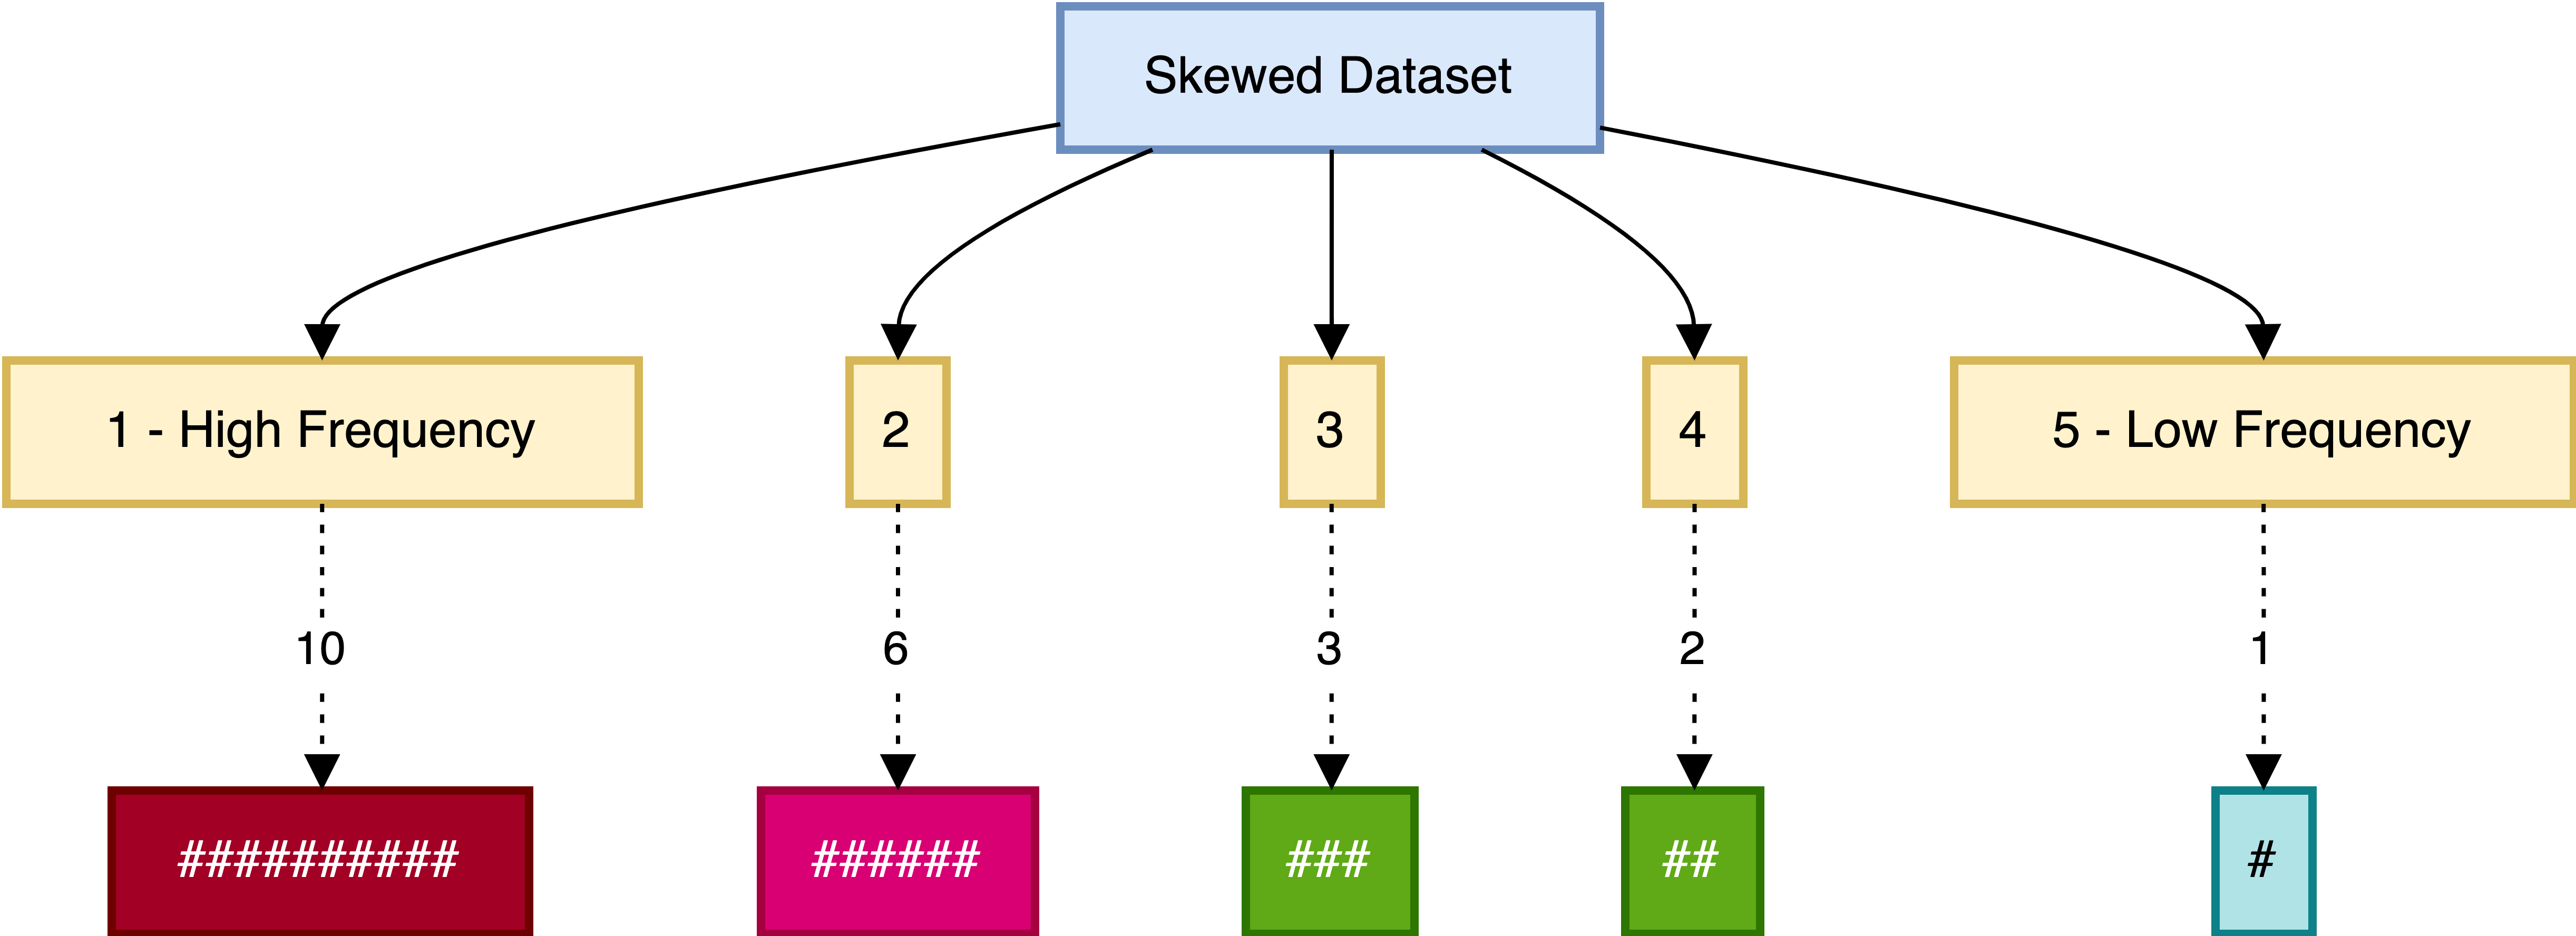
\includegraphics[width=\textwidth,height=.7\textheight,keepaspectratio]{./Figures/chapter-03/dwh_hive-skweed_dt.png}	
					\caption{Abstract Components of Apache Hive}
				\end{figure}
			\end{tcolorbox}
		\end{frame}

		\begin{frame}[fragile]
			\frametitle{CREATE TABLE in Hive | continued}    
			\vspace{-0.5cm}		
			\begin{tcolorbox}[colback=white,colframe=black,title= Part 7: Data Skewing]
	
		% The 'axis' environment is used to draw the histogram.
			\begin{figure} % 'h' places the figure approximately here
			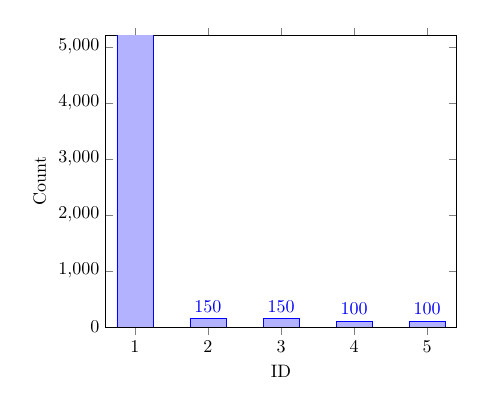
\begin{tikzpicture}[scale=0.65]
				\begin{axis}[
					ybar,
					ymin=0, % The minimum value on the y-axis.
					ymax=5200, % Adjust the maximum value according to your needs.
					symbolic x coords={1,2,3,4,5}, % X-axis coordinates.
					xtick=data, % Define ticks on the x-axis based on data points.
					nodes near coords, % Place nodes near the coordinates.
					nodes near coords align={vertical}, % Align the nodes vertically.
					xlabel={ID}, % Label for the x-axis.
					ylabel={Count}, % Label for the y-axis.
					bar width=20pt, % The width of the bars.
				]
				\addplot coordinates {(1,50000) (2,150) (3,150) (4,100) (5,100)}; % Data points for the plot.
				\end{axis}
			\end{tikzpicture}
			\caption{Data Skewing Example: ID Frequency histogram} % Add your caption
    		\label{fig:ch_3_hive_skewness_histogram} % Optional: For referencing the figure in text
			\end{figure}
			\end{tcolorbox}
		\end{frame}
		\begin{frame}
			\frametitle{CREATE TABLE in Hive | continued}  
			\vspace{-0.5cm}		
			\begin{tcolorbox}[colback=white,colframe=black,title= Part 7: Data Skewing]	
				\vspace{-0.3cm}
				\begin{figure}
					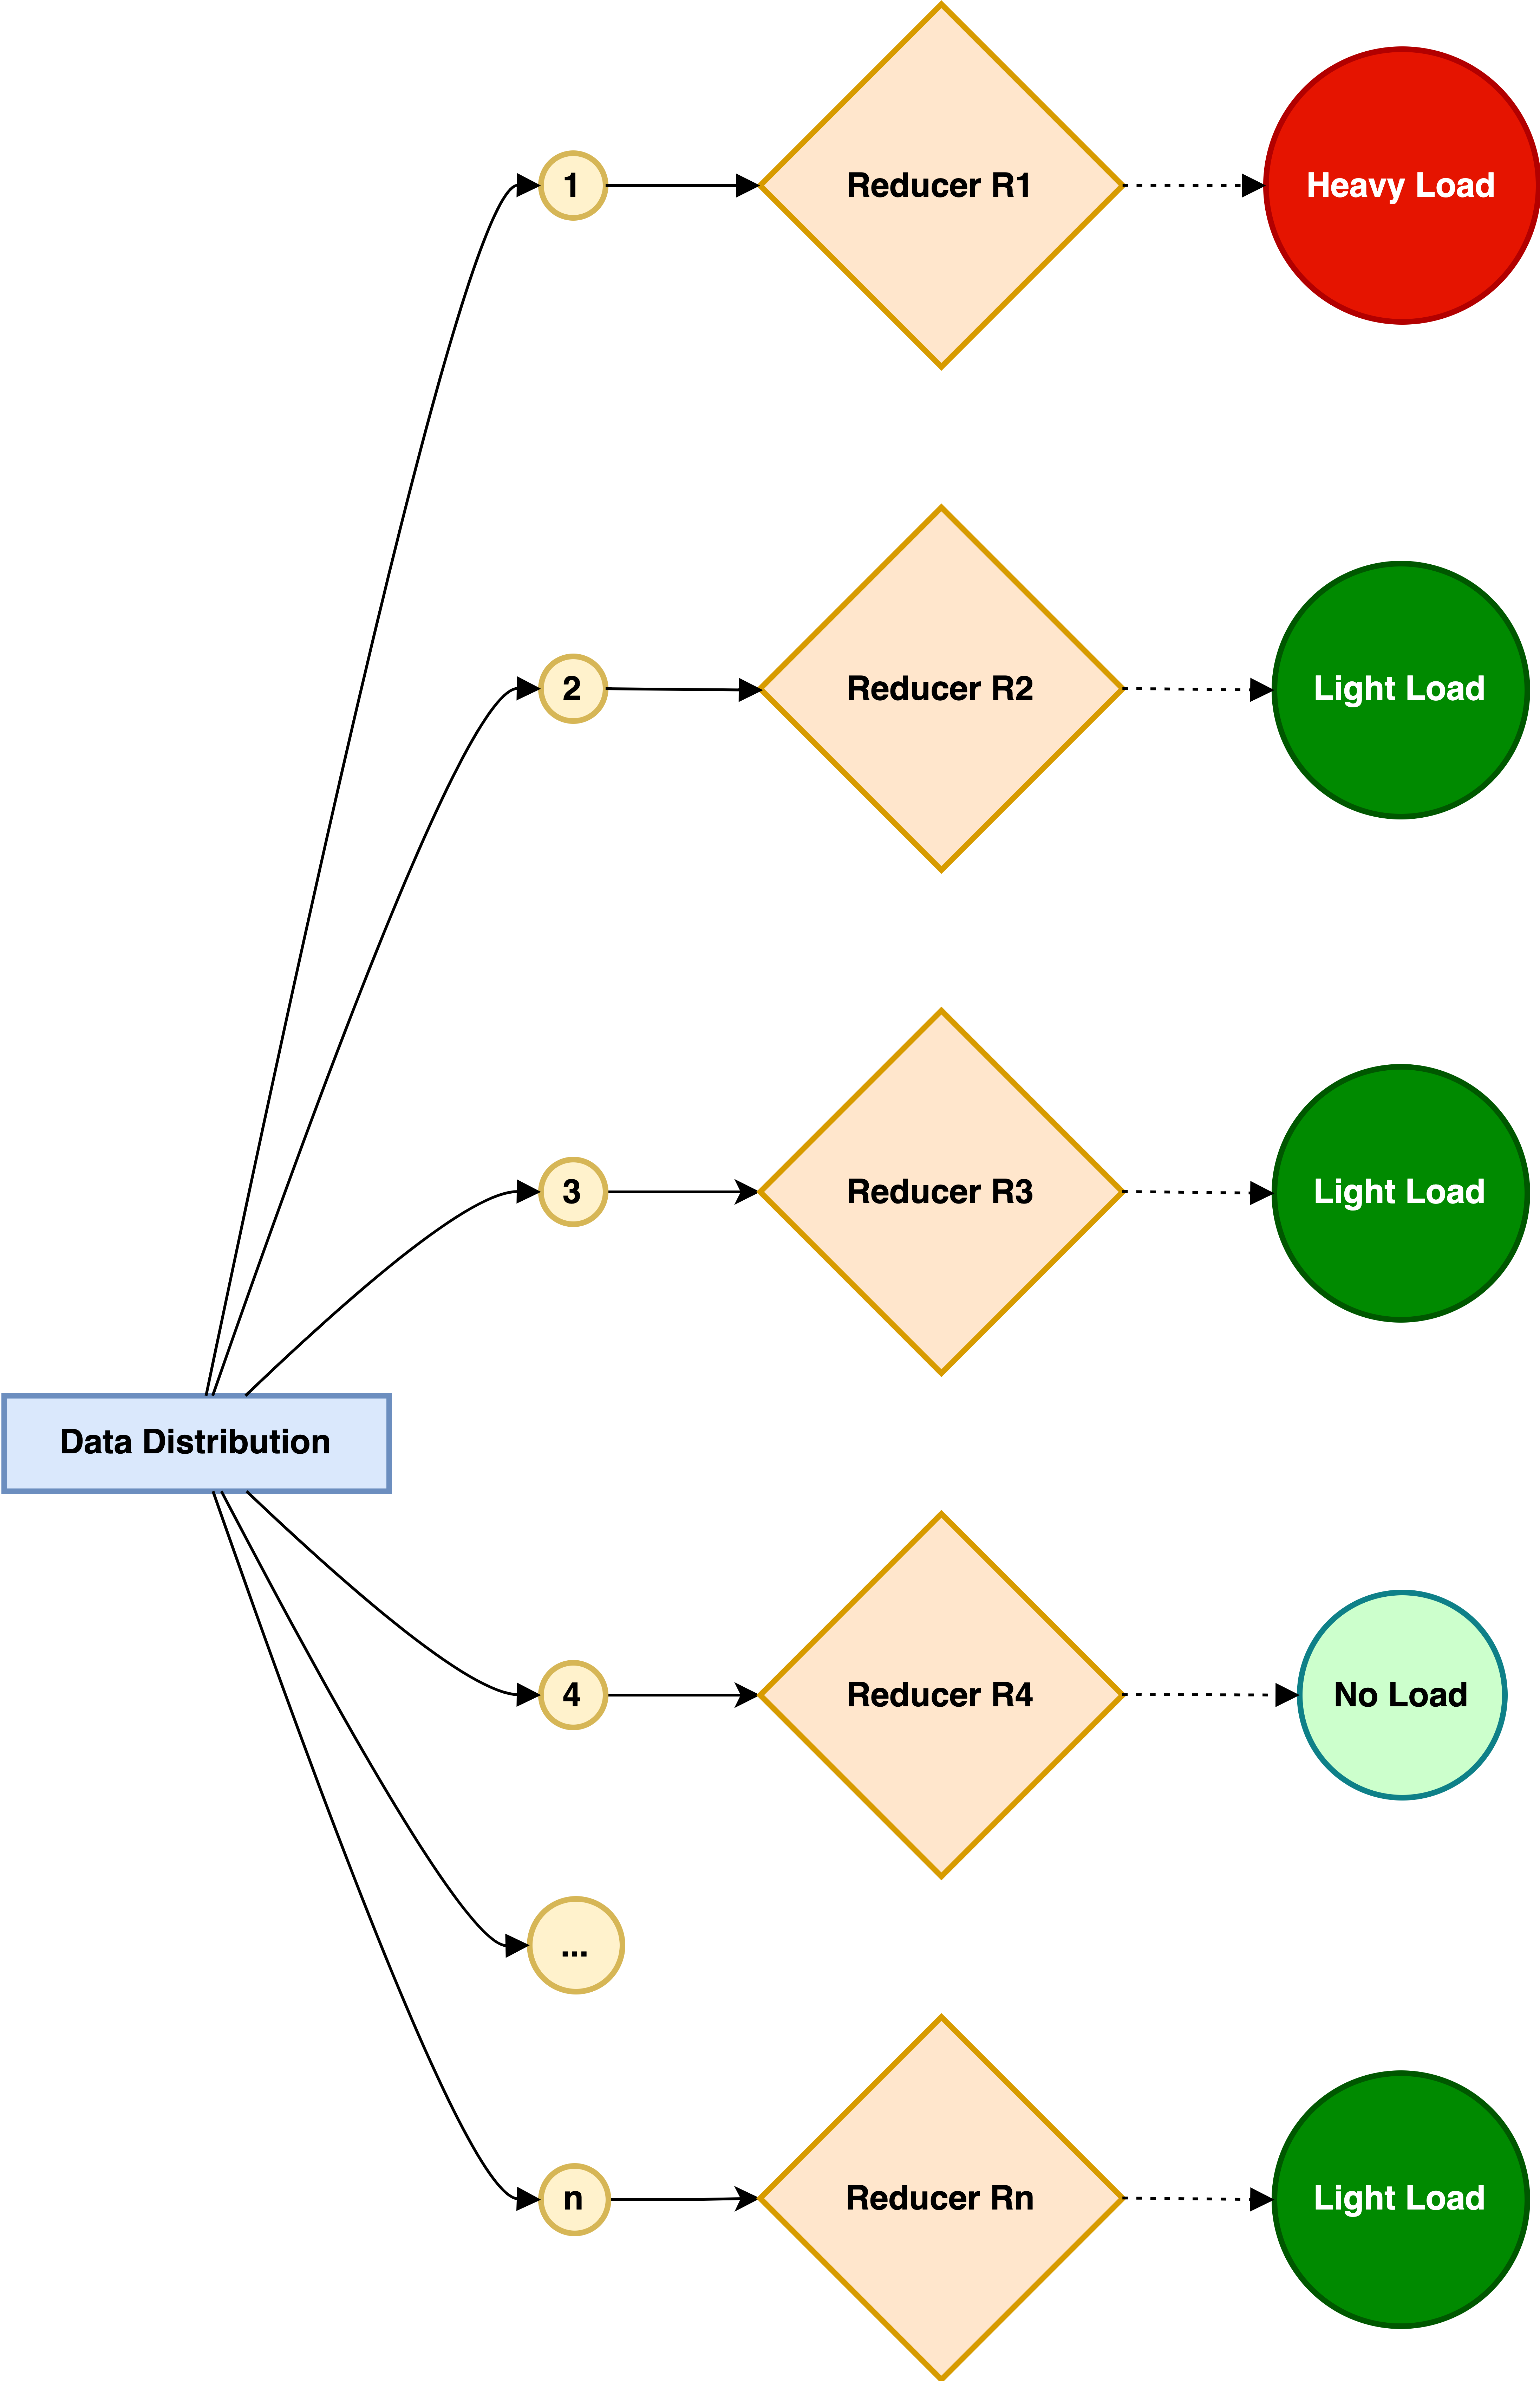
\includegraphics[width=\textwidth,height=.7\textheight,keepaspectratio]{./Figures/chapter-03/dwh_hive-skweed_dt_mr_2.png}	
					\caption{Abstract Components of Apache Hive}
				\end{figure}
				\vspace{-0.3cm}
			\end{tcolorbox}
		\end{frame}		
		\begin{frame}
			\frametitle{CREATE TABLE in Hive | continued}  
			\vspace{-0.5cm}		
			\begin{tcolorbox}[colback=white,colframe=black,title= Part 7: Data Skewing]					
				\begin{figure}
					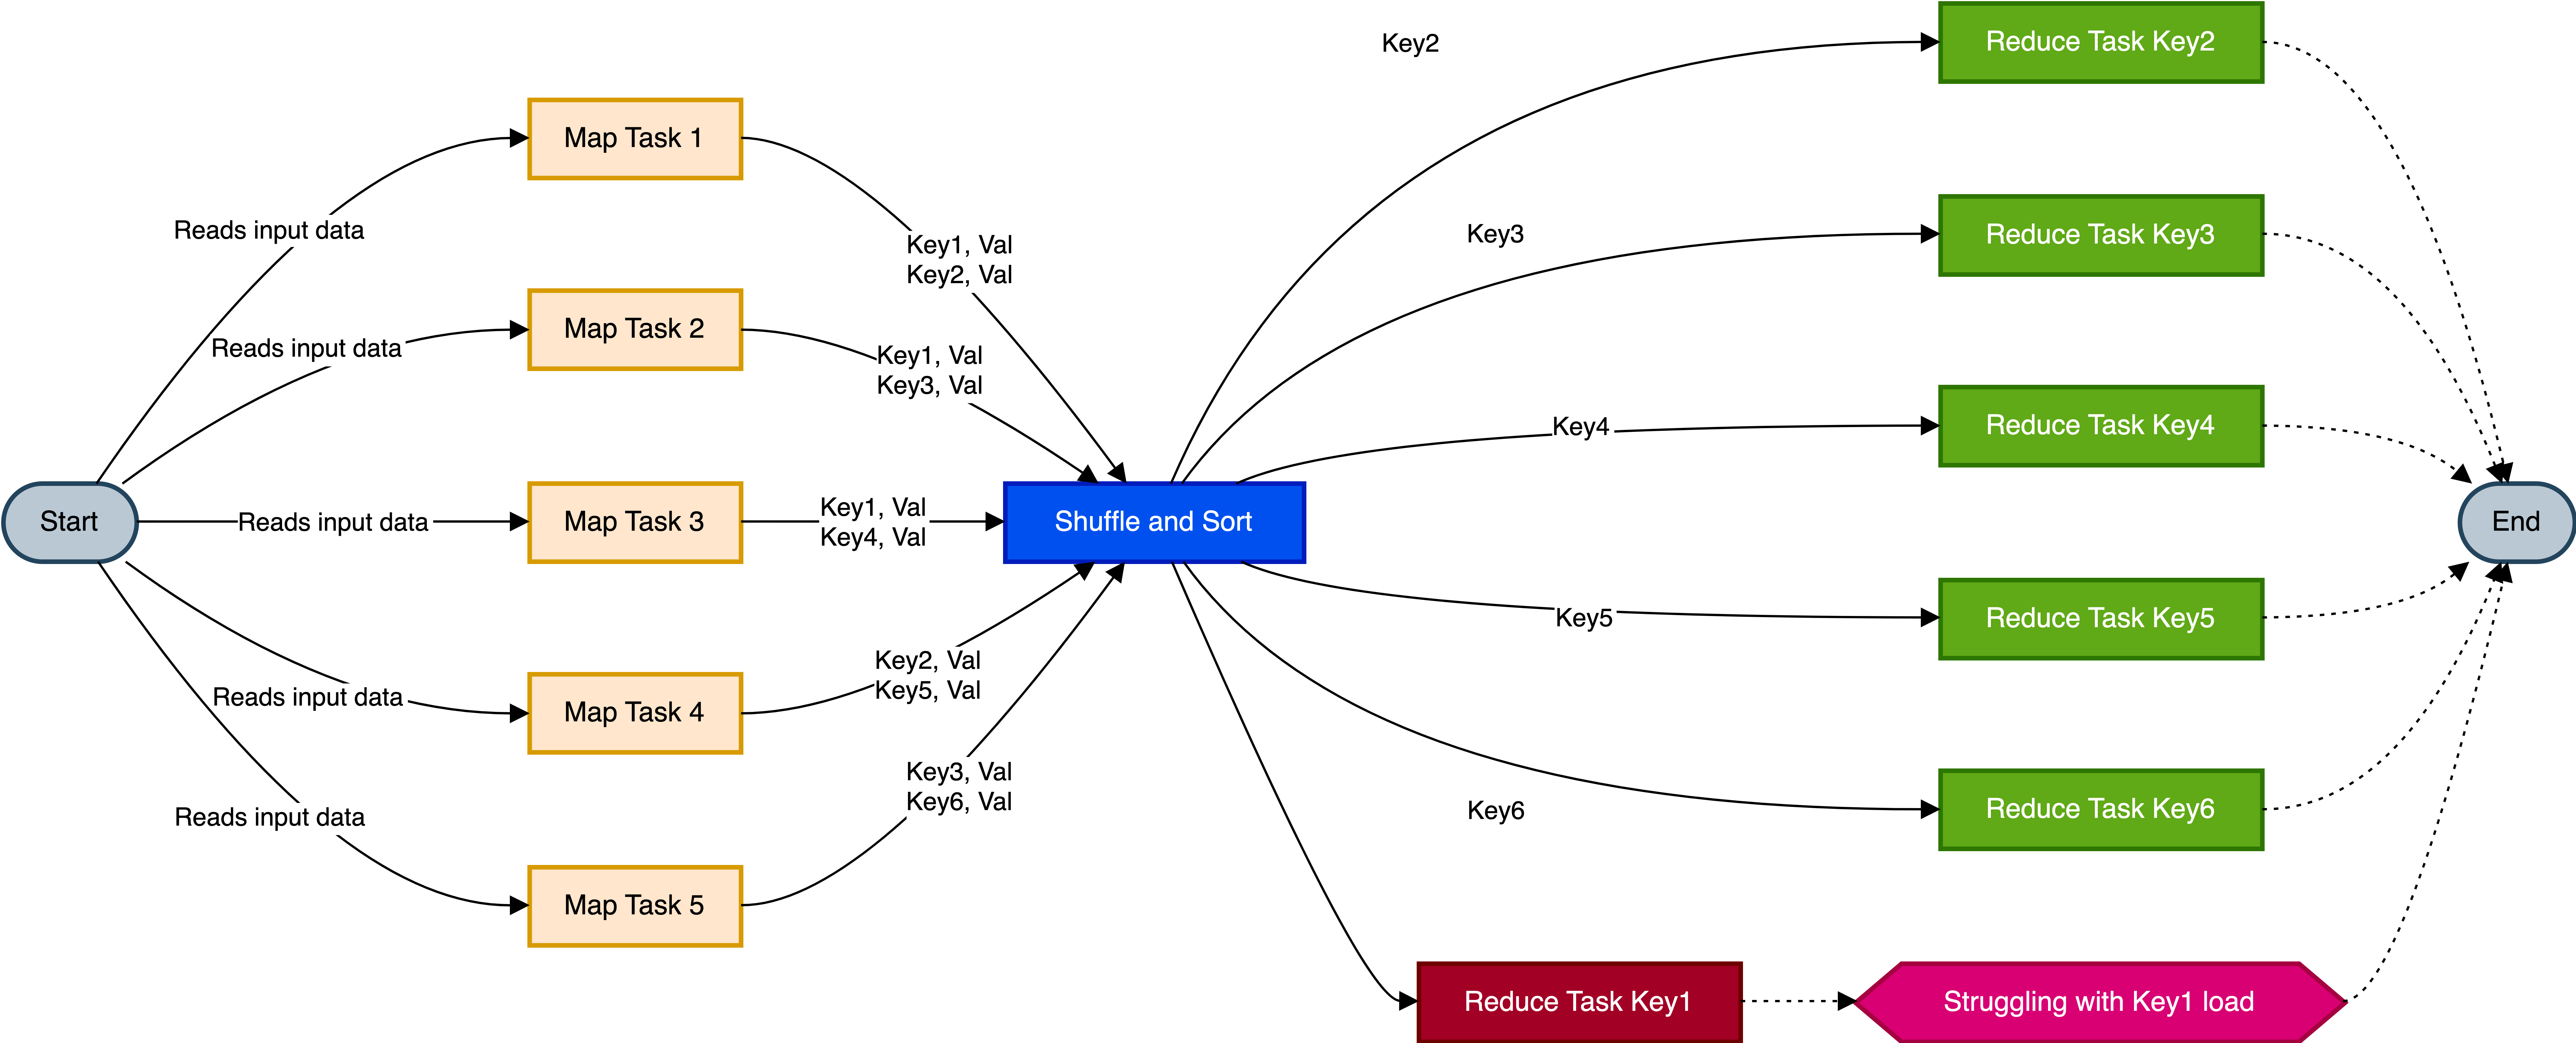
\includegraphics[width=\textwidth,height=.7\textheight,keepaspectratio]{./Figures/chapter-03/dwh_hive-skweed_dt_mr.png}	
					\caption{Abstract Components of Apache Hive}
				\end{figure}
			\end{tcolorbox}
		\end{frame}	
		
		\begin{frame}
			\frametitle{CREATE TABLE in Hive | continued}  
			\vspace{-0.5cm}		
			\begin{tcolorbox}[colback=white,colframe=black,title= Part 7: Data Skewing]	
				\begin{figure}
					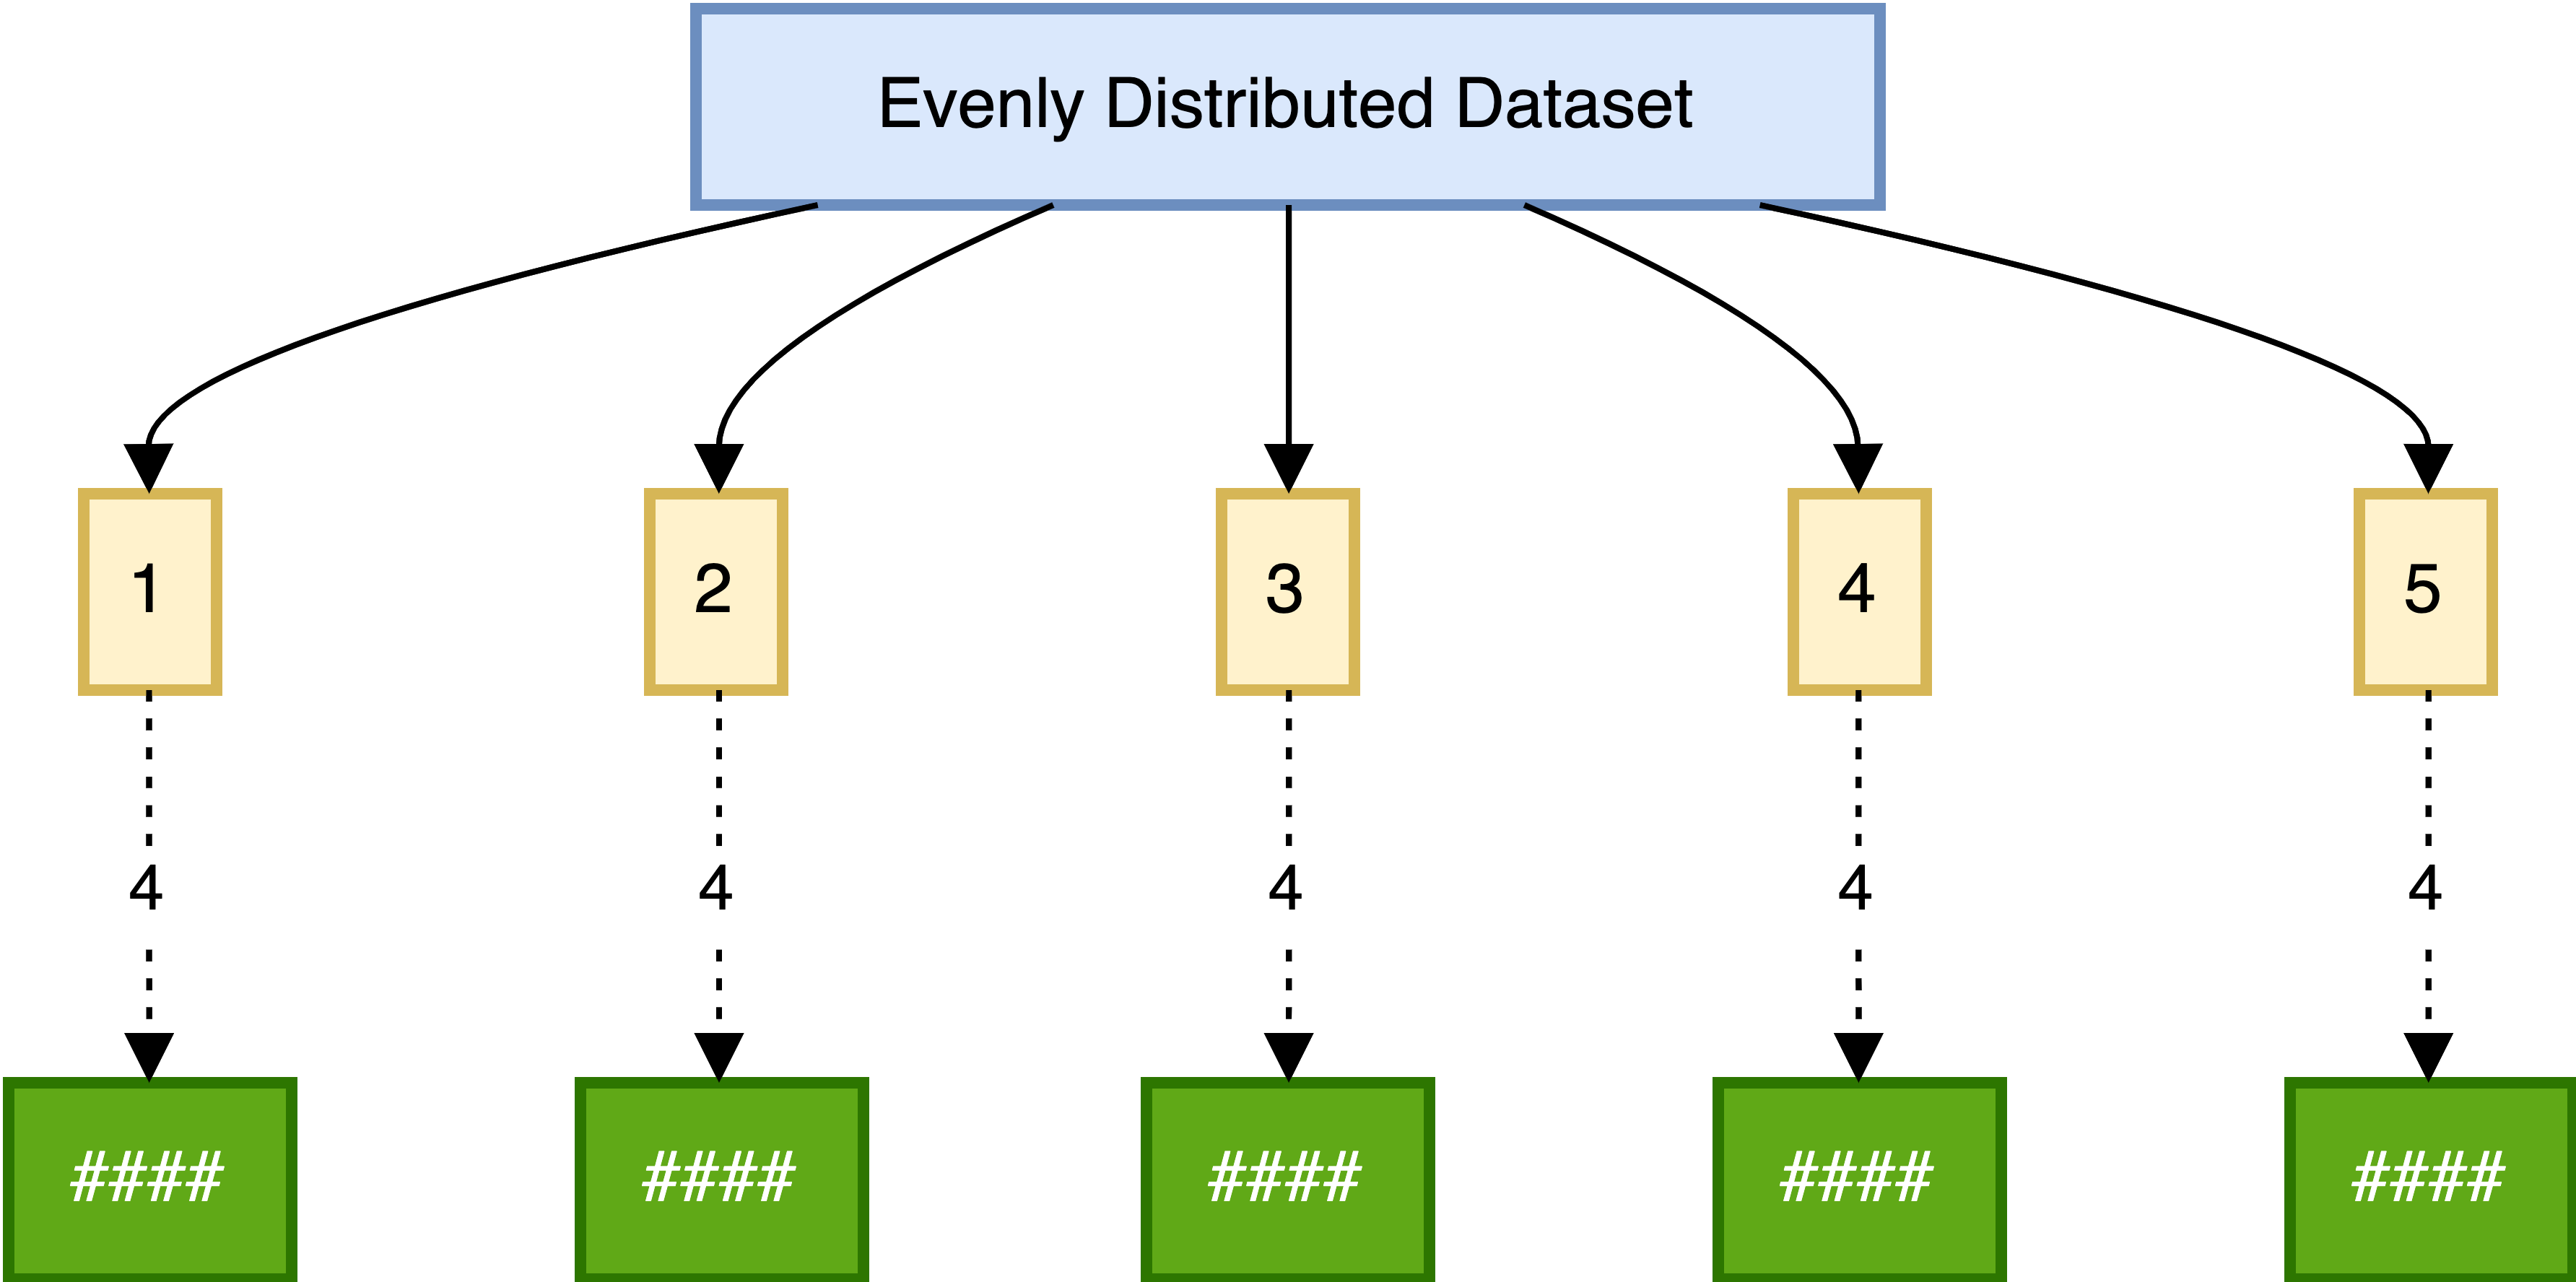
\includegraphics[width=\textwidth,height=.6\textheight,keepaspectratio]{./Figures/chapter-03/dwh_hive-unskweed_dt.png}	
					\caption{Abstract Components of Apache Hive}
				\end{figure}
			\end{tcolorbox}
		\end{frame}
		\begin{frame}
			\frametitle{CREATE TABLE in Hive | continued}  
			\vspace{-0.5cm}		
			\begin{tcolorbox}[colback=white,colframe=black,title= Part 7: Data Skewing]	
				\begin{figure}
					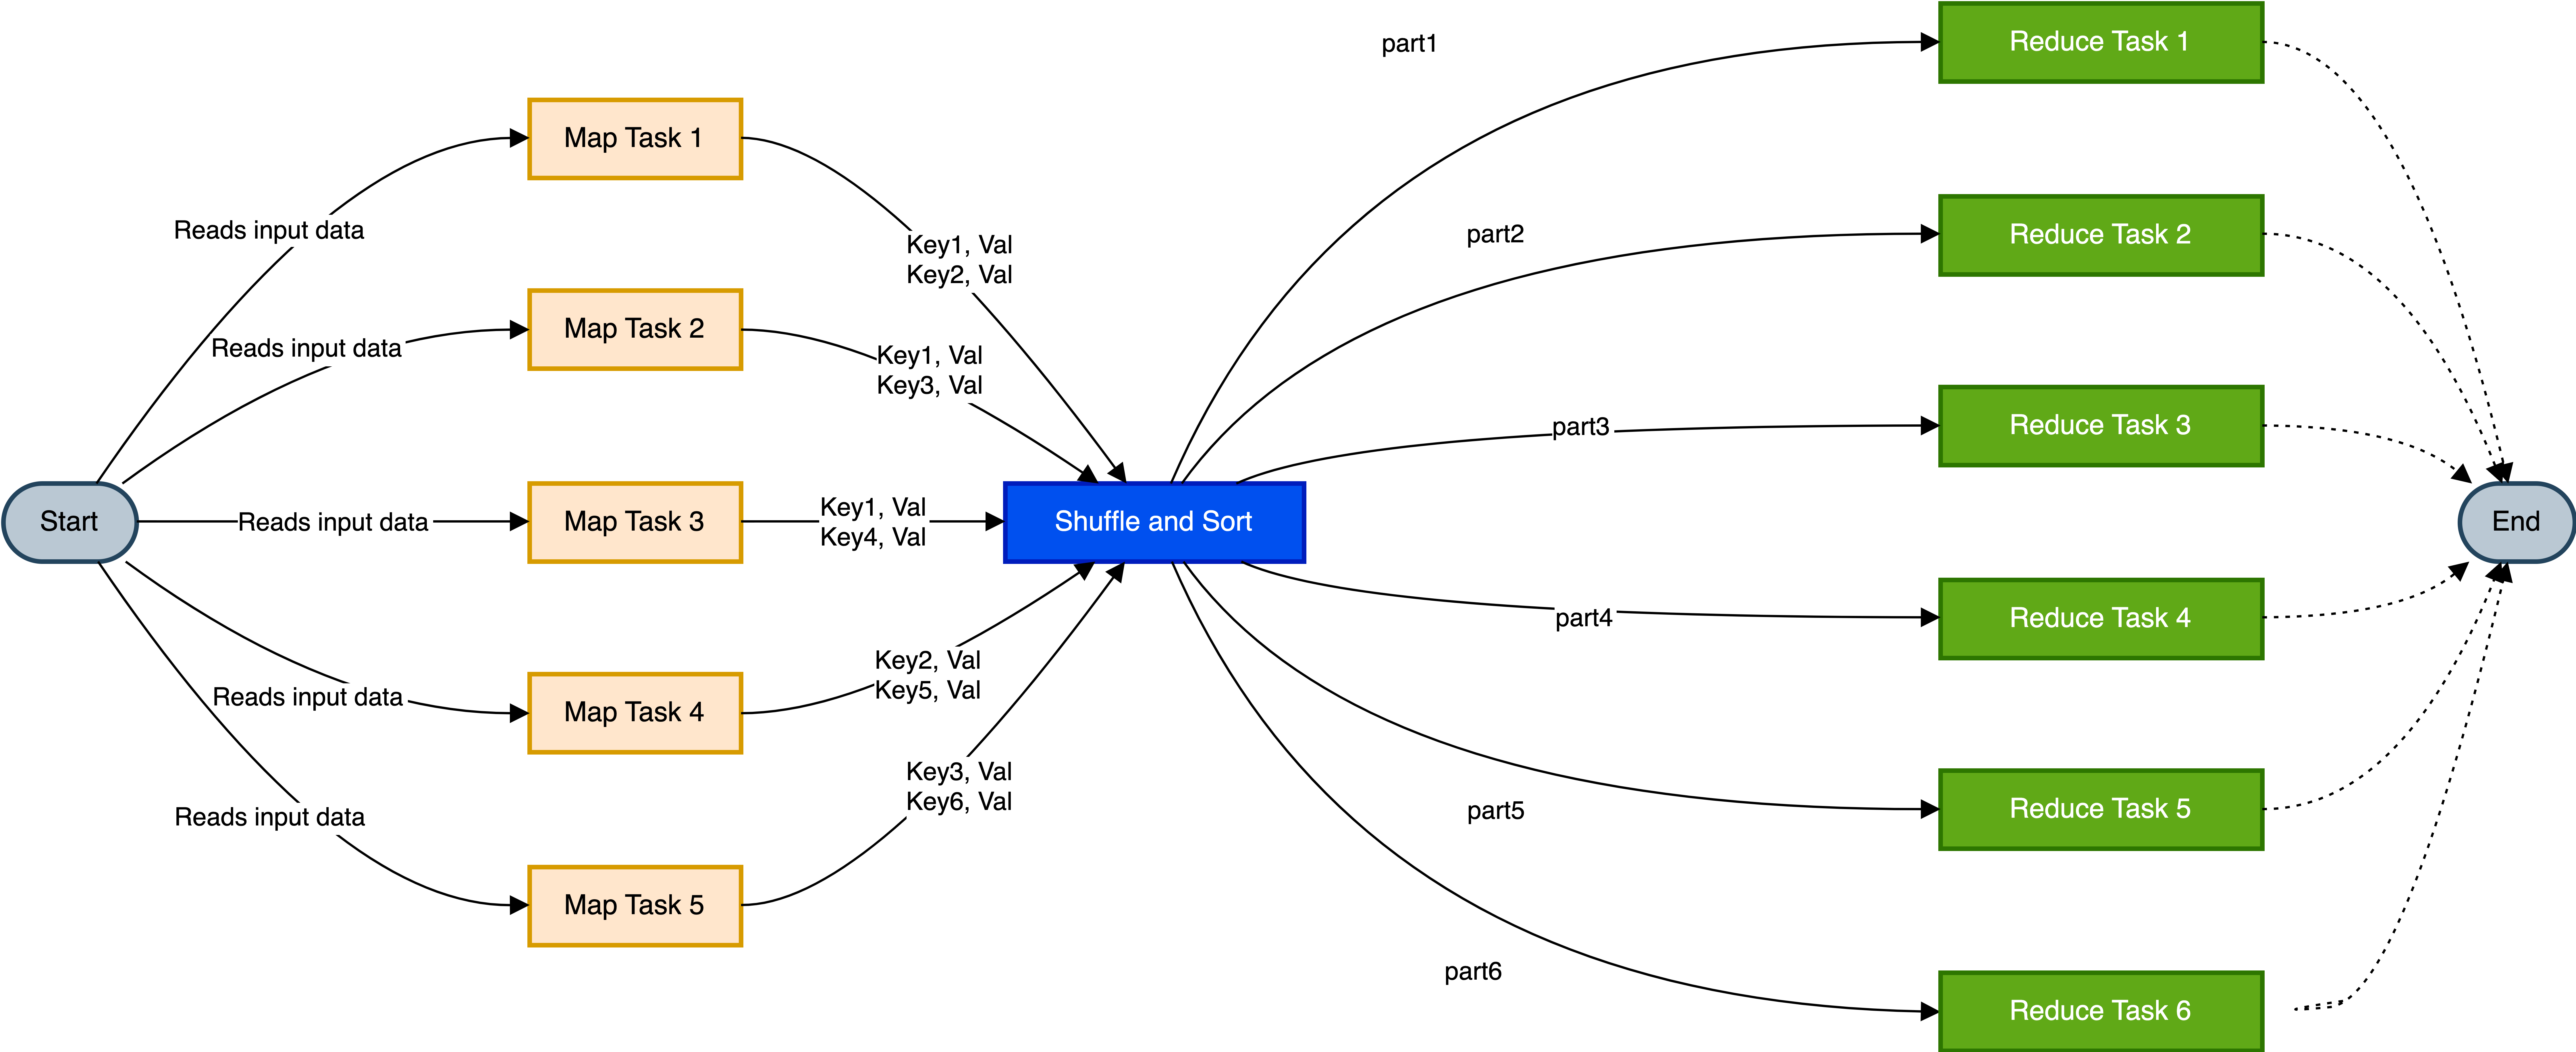
\includegraphics[width=\textwidth,height=.7\textheight,keepaspectratio]{./Figures/chapter-03/dwh_hive-unskweed_dt_mr.png}	
					\caption{Abstract Components of Apache Hive}
				\end{figure}
			\end{tcolorbox}
		\end{frame}	
		
		\begin{frame}{CREATE TABLE in Hive | continued}
			\begin{tcolorbox}[colback=white,colframe=black,title= Part 8: Table Location]
				\small
				\begin{itemize}
			  		\item \textbf{Resolving Skewness with Hive's \texttt{SKEWED BY} }
			  		\begin{itemize}
						\item When a table is created in Hive, you can specify certain columns as \texttt{'SKEWED BY'} to improve the distribution of work during a join operation. This allows Hive to partition the data more effectively.
			  		\end{itemize}
				\end{itemize}
			\end{tcolorbox}	
		\end{frame}
	
 \begin{frame}{CREATE TABLE in Hive | continued}
	\begin{tcolorbox}[colback=white,colframe=black,title= Part 8: Table Location]
		\small
		\begin{itemize}
			\item \texttt{[LOCATION hdfs\_path]}
			\begin{itemize}
				\item Sets the HDFS directory where table data will be stored.
			\end{itemize}
		\end{itemize}
	\end{tcolorbox}	
\end{frame}
  
  \begin{frame}{CREATE TABLE in Hive | continued}
	\begin{tcolorbox}[colback=white,colframe=black,title= Part 9: Table Properties]
		\small
	\begin{itemize}
	  \item \texttt{[TBLPROPERTIES (property\_name=property\_value, ...)]}
	  \begin{itemize}
		\item Sets table-level properties.
	  \end{itemize}
	\end{itemize}
	\end{tcolorbox}
  \end{frame}
  
  \begin{frame}{CREATE TABLE in Hive | continued}
	\begin{tcolorbox}[colback=white,colframe=black,title= Part 10: CTAS]
		\small
	\begin{itemize}
	  \item \texttt{[AS select\_statement]}
	  \begin{itemize}
		\item Populates the table using the result set of a SELECT statement.
	  \end{itemize}
	\end{itemize}
	\end{tcolorbox}
  \end{frame}
   












































%%%%%%%%%%%%%%%%%%%%%%%%%%%%%%%%%%%%%%%%%%%%%%%%%%%%%%
\subsubsection{Query Execution Plan}
\begin{frame}
	\frametitle{Query Execution Plan}
	\framesubtitle{Overview}
	
	\begin{itemize}
	  \item The Hive driver is responsible for translating SQL statements into an execution plan for the target execution engine.
	  \item The process involves several key steps:
		\begin{enumerate}
		  \item The parser parses the SQL statement and generates an Abstract Syntax Tree (AST) representing logical operations like SELECTs, JOINs, UNIONs, groupings, and more.
		  \item The planner retrieves table metadata from the Hive Metastore, including HDFS file locations, storage formats, row counts, etc.
		  \item The query optimizer utilizes the AST and table metadata to produce a physical operation tree known as the execution plan, defining the physical operations needed to retrieve data, such as nested loop joins, sort-merge joins, hash joins, index joins, and more.
		\end{enumerate}

	\end{itemize}
	
	\end{frame}
	
	\begin{frame}
	\frametitle{Query Execution Plan}
	\framesubtitle{Impact on Performance}
	
	\begin{itemize}
	\item The execution plan determines the tasks executed on the Hadoop cluster and significantly impacts performance in data analytics systems like Hive.
	  \item The execution plan generated by the query optimizer has a substantial impact on performance.
	  \item Differences in the execution plan can result in significant variations in execution time, ranging from seconds to hours.
	  \item An optimal execution plan is crucial for efficient query processing in Hive.
	\end{itemize}
	
	\end{frame}
	
	\begin{frame}
	\frametitle{Query Execution Plan}
	\framesubtitle{Cost-Based Optimization (CBO)}
	
	\begin{itemize}
	  \item The Cost-Based Optimization (CBO) plays a pivotal role in enhancing the execution plan.
	  \item CBO leverages table statistics to make informed decisions regarding the performance costs associated with each potential execution plan.
	  \item This intelligent optimization ensures that the Hive driver produces an optimal execution plan, improving query performance.
	\end{itemize}
	
	\end{frame}
\subsubsection{Cost-Based Optimization}
%%%%%%%%%%%%%%%%%%%%%%%%%%%%%%%%%%%%%%%%%%%%%%%%%%%%%%%%%%%%%%%%%%%%%%%%%%%


%%%%%%%%%%%%%%%%%%%%%%%%%%%%%%%%%%%%%%%%%%%%%%%%%%%%%%
\subsubsection{Hive Schema and Data Storage}
\begin{frame}{Hive Schema and Data Storage}
	\begin{itemize}
		\item Hive queries operate on tables, similar to RDBMS.
		\begin{itemize}
			\item A table corresponds to a directory in storage (HDFS, S3, GCS, or Azure).
			\item Each table comprises one or more files.
			\item Every table is associated with a specific file format.
			\item Hive stores table structure and location in the metadata store (RDBMS).
			\item Hive supports various file formats, such as Parquet, ORC, and Text.
		\end{itemize}
	\end{itemize}
\end{frame}

\begin{frame}{Hive Schema and Data Storage (Continued)}
	\begin{itemize}
		\item Hive queries reference the metastore to access table location and structure.
		\item While queries interact with the file system, metadata is stored in the RDBMS.
	\end{itemize}
\end{frame}
%%%%%%%%%%%%%%%%%%%%%%%%%%%%%%%%%%%%%%%%%%%%%%%%%%%%%%%%%%%%%%%%%%%%%%%%%%%
\subsection{Further Readings and Assignment}

%%% Local Variables:
%%% mode: latex
%%% TeX-master: "../main"
% !TeX root = ../main.tex
%%% TeX-engine: xetex
%%% End: